\documentclass[11pt,class=report,crop=false]{standalone}
\usepackage[screen]{../mathgame}

% Commenter pour afficher les figures longuettes à calculer !!
%\renewcommand{\commentfigure}[1]{\mybox{\emph{Ici une figure.}}}  % sans les figures compliquées

\begin{document}


%====================================================================
\chapitre{Perspective}
%====================================================================

%
%\insertvideo{yUgpElITYTg}{partie 5.1. Bits classiques}
%
%\insertvideo{iET0snUXj0k}{partie 5.2. Portes logiques}
%
%\insertvideo{JKmC2u5kvKg}{partie 5.3. Algorithme et complexité}

\objectifs{Nous expliquons différentes façons de représenter l'espace 3D sur un plan 2D.}

%%%%%%%%%%%%%%%%%%%%%%%%%%%%%%%%%%%%%%%%%%%%%%%%%%%%%%%%%%%%%%%%%%%%%
\section{Perspective linéaire}

\index{perspective!lineaire@linéaire}

La perspective linéaire est aussi appelée \emph{perspective conique} ou \emph{projection centrale}.

%--------------------------------------------------------------------
\subsection{Principe}

La perspective linéaire est la perspective qui se rapproche le plus de la vision humaine, les objets éloignés paraissent plus petits.

Notations :
\begin{itemize}
  \item $C$ est un point de l'espace, il peut représenter la caméra, l'\oe{}il, un capteur, ou aussi un éclairage,
  \item $\mathcal{P}$ est un plan de l'espace,
  \item $P$ désigne un point d'un objet $\mathcal{O}$.
\end{itemize}

Construction : pour chaque point $P$, si la droite $(CP)$ recoupe le plan $\mathcal{P}$, on note $P'$ ce point d'intersection. On définit ainsi une projection de
l'espace $\mathcal{E}$ sur le plan $\mathcal{P}$.

\myfigure{0.8}{\tikzinput{fig-perspective-01}}

Voici quelques projections du même cube mais avec différents points $C$.

\myfigure{1}{\tikzinput{fig-perspective-01a}}


%--------------------------------------------------------------------
\subsection{Cas simple}

L'espace est muni du repère orthonormé $(Oxyz)$ classique.
Le point $C(f,0,0)$ est fixé sur l'axe $(Ox)$ (la valeur $f$ s'appelle la \emph{focale}).
Le plan $\mathcal{P}$ de projection est le plan $(Oyz)$, c'est-à-dire d'équation $(x=0)$. Dans ce plan on note $(X,Y)$ les coordonnées du plan (avec $X=y$ et $Y=z$).

\myfigure{0.7}{
	\tikzinput{fig-perspective-03a}\qquad\qquad
    \tikzinput{fig-perspective-03b}
}


\begin{proposition}
Pour $P$ de coordonnées $(x,y,z)$ (avec $x \neq f$) alors son image par la perspective linéaire est $P'$ de coordonnées $(X,Y)$ dans $\mathcal{P}$ avec :
\mybox{$\displaystyle
\left\{\begin{array}{rcl}
X &=& \lambda y \\
Y &=& \lambda z \\
\end{array}\right.
\qquad \text{ où }\qquad
\lambda = \frac{-f}{x-f}
$}
\end{proposition}


\begin{proof}
Les points $C$, $P$ et $P'$ sont alignés donc il existe $\lambda \in \Rr$ tel que $\overrightarrow{CP'} = \lambda \overrightarrow{CP}$.
Notons $P'(0,y',z')$ les coordonnées de $P'$ dans le repère $(Oxyz)$. Alors :
$$
\overrightarrow{CP} = \begin{pmatrix}x-f\\y\\z\end{pmatrix}
\qquad\qquad
\overrightarrow{CP'} = \begin{pmatrix}-f\\y'\\z'\end{pmatrix}$$
Ainsi
$$\overrightarrow{CP'} = \lambda \overrightarrow{CP}
\iff
\left\{\begin{array}{rcl}
-f &=& \lambda (x-f) \\
y'  &=& \lambda y \\
z' &=& \lambda z \\
\end{array}\right.
\iff
\left\{\begin{array}{rcl}
\lambda &=&  \frac{-f}{x-f} \\
X &=& \lambda y \\
Y &=& \lambda z \\
\end{array}\right.$$
où l'on a identifié $X=y'$ et $Y=z'$.
\end{proof}

%--------------------------------------------------------------------
\subsection{Cas général}

Voici les formules, pour le cas d'un point $C(x_C,y_C,z_C)$ de coordonnées quelconques, en projetant toujours sur le plan $(Oyz)$, 
\begin{proposition}
Pour $P$ de coordonnées $(x,y,z)$ (avec $x \neq x_C$) alors son image par la perspective linéaire est $P'$ de coordonnées $(X,Y)$ dans $\mathcal{P}$ avec :
\mybox{$\displaystyle
\left\{\begin{array}{rcl}
X &=& \lambda (y-y_C) + y_C \\
Y &=& \lambda (z-z_C) + z_C \\
\end{array}\right.
\qquad \text{ où }\qquad
\lambda = \frac{-x_C}{x-x_C}
$}
\end{proposition}

\begin{proof}
Depuis l'identité $\overrightarrow{CP'} = \lambda \overrightarrow{CP}$, on a :
$$
\begin{pmatrix}0-x_C\\y'-y_C\\z'-z_C\end{pmatrix}
= \lambda 
\begin{pmatrix}x-x_C\\y-y_C\\z-z_C\end{pmatrix},$$
d'où les formules.
\end{proof}


%%%%%%%%%%%%%%%%%%%%%%%%%%%%%%%%%%%%%%%%%%%%%%%%%%%%%%%%%%%%%%%%%%%%%
\section{Projection orthogonale}

\index{projection!orthogonale}

%--------------------------------------------------------------------
\subsection{Principe}

C'est comme si on plaçait une caméra à une distance infinie, dirigée orthogonalement à un plan.
Une fois projetés, deux objets identiques auront les mêmes dimensions, qu'ils soient proches ou éloignés du plan de projection.
La projection orthogonale est utilisée  dans le dessin technique, les plans d'architectes\ldots


\myfigure{1}{\tikzinput{fig-perspective-02}}


Voici quelques projections obtenues en faisant tourner un cube.
\myfigure{1}{\tikzinput{fig-perspective-02a}}

%--------------------------------------------------------------------
\subsection{Cas simple}


Le plan de projection $\mathcal{P}$ est le plan $(Oyz)$ et l'axe de projection est l'axe $(Ox)$. Le vecteur $\vec n = \left(\begin{smallmatrix}1\\0\\0\end{smallmatrix}\right)$ est colinéaire à cet axe et orthogonal au plan.

\myfigure{1}{\tikzinput{fig-perspective-04}}

Si on considère la projection comme une application de $\Rr^3 \to \Rr^3$ alors elle s'écrit :
$$P =  \begin{pmatrix}x\\y\\z\end{pmatrix} \longmapsto P' =  \begin{pmatrix}0\\y\\z\end{pmatrix}.$$
C'est une application linéaire, dont la matrice est :
$$M_1 = 
\begin{pmatrix}
0&0&0\\
0&1&0\\
0&0&1\\
\end{pmatrix}.
$$


Si on considère cette projection de l'espace vers le plan $\mathcal{P}$ dont les coordonnées sont $(X,Y)$, alors les formules sont tout simplement :
 $$X=y \qquad \text{ et } \qquad Y=z.$$
La matrice correspondante est :
$$
M_1' = \begin{pmatrix}
0&1&0\\
0&0&1\\
\end{pmatrix}.
$$

%--------------------------------------------------------------------
\subsection{Cas général}

On considère une projection orthogonale sur un plan quelconque (passant par l'origine). Ce plan est déterminé par un vecteur normal $\vec n$, qui est aussi la direction de projection. 
Nous allons caractériser cette direction par un vecteur déterminé par ses coordonnées longitude/latitude. Ainsi une projection orthogonale est déterminée par le vecteur $\vec n = \overrightarrow{OM}$ où le point $M(1,\varphi,\lambda)$ est défini en coordonnées sphériques (par sa latitude $\varphi$ et sa longitude $\lambda$).


\commentfigure{
	\myfigure{0.8}{\tikzinput{fig-perspective-05}}
}

On note $(X,Y)$ les coordonnées sur le plan de projection.

\begin{proposition}
La projection orthogonale suivant l'axe de latitude $\varphi$ et de longitude $\lambda$ est donnée par l'application : 
$\left(\begin{smallmatrix}x\\y\\z\end{smallmatrix}\right)
\mapsto \left(\begin{smallmatrix}X\\Y\end{smallmatrix}\right)$ définie par :
$$\begin{pmatrix}X\\Y\end{pmatrix} = M \begin{pmatrix}x\\y\\z\end{pmatrix}
\qquad \text{ où } \qquad 
M = \begin{pmatrix}
-\sin\lambda & \cos\lambda & 0\\
\sin\varphi\cos\lambda&\sin\varphi\sin\lambda&\cos\varphi\\
\end{pmatrix}.
$$
Autrement dit :
$$\left\{
\begin{array}{rcl}
X &=& -\sin(\lambda) \cdot x + \cos(\lambda) \cdot y \\
Y &=& \sin(\varphi)\cos(\lambda) \cdot x +\sin(\varphi)\sin(\lambda) \cdot y + \cos(\varphi) \cdot z \\
\end{array}
\right.$$
\end{proposition}


\begin{proof}
Il s'agit de se ramener au cas simple, c'est-à-dire à la projection orthogonale sur le plan $(Oyz)$ dont la matrice est $M_1'$.

\begin{itemize}
  \item Tout d'abord on modifie le plan de projection, en changeant la longitude de sorte que la trace du plan de projection sur le plan horizontal $(Oxy)$ soit l'axe $(Oy)$. L'opération correspondante est une rotation d'angle $-\lambda$ autour de l'axe $(Oz)$. La matrice de cette opération est :
  $$M_3 = 
  \begin{pmatrix}
  \cos\lambda & \sin\lambda & 0\\
  -\sin\lambda & \cos\lambda & 0\\
  0&0&1\\
  \end{pmatrix}.
  $$


\myfigure{0.6}{\tikzinput{fig-perspective-06}}

  \item Ensuite on redresse le plan à la verticale en modifiant la latitude $\varphi$ (de façon à ce que le plan contienne l'axe $(Oz)$).
  Il s'agit d'effectuer une rotation d'angle $-\varphi$ autour de l'axe $(Oy)$.
  La matrice de cette transformation est :
  $$M_2 = 
  \begin{pmatrix}
  \cos\varphi & 0 & -\sin\varphi \\
   0&1&0\\
  \sin\varphi & 0 & \cos\varphi\\
  \end{pmatrix}.
  $$
  

  \item Le plan de projection est devenu le plan $(Oyz)$, il ne reste alors plus qu'à projeter suivant l'axe $(Ox)$, la matrice de cette projection est la matrice $M_1'$ du cas simple. 

  \item Les formules s'obtiennent par composition : 
  $$\begin{pmatrix}X\\Y\end{pmatrix} = M \begin{pmatrix}x\\y\\z\end{pmatrix} 
  \qquad \text{ où } \qquad 
  M = M_1' M_2 M_3.
  $$
\end{itemize}

\end{proof}

\emph{Remarque.} Si on veut les coordonnées $\left(\begin{smallmatrix}x'\\y'\\z'\end{smallmatrix}\right)$ du projeté $P'$ dans les coordonnées originales $(Oxyz)$, les formules sont :
$$\begin{pmatrix}x'\\y'\\z'\end{pmatrix} 
= (M_2 M_3)^{-1} M_1  (M_2 M_3)
\begin{pmatrix}x\\y\\z\end{pmatrix}.$$


%--------------------------------------------------------------------
\subsection{Cas particuliers}

Des valeurs classiques sont :
\begin{itemize}
  \item $\lambda = \ang{30}$ et $\varphi = \ang{20}$,
  \item $\lambda = \frac\pi4 = \ang{45}$ et différentes valeurs de $\varphi$. 
\end{itemize}

\begin{exemple}[Perspective isométrique]
 
Les paramètres sont $\lambda = \frac\pi4 = \ang{45}$ et $\varphi$ tel que $\sin\varphi = \frac{1}{\sqrt3}$ (de sorte que $\varphi \simeq \ang{35}$).
Pour la perspective isométrique les trois axes ont la même importance (mais ce n'est pas une isométrie au sens géométrique usuel).
Le vecteur normal au plan de projection est $\left(\begin{smallmatrix}1\\1\\1\end{smallmatrix}\right)$.


\myfigure{1.5}{
	\tikzinput{fig-perspective-07}\qquad\qquad
    \tikzinput{fig-perspective-08}
}

La matrice de cette projection est :
$$\begin{pmatrix}
-\frac{\sqrt2}{2} & \frac{\sqrt2}{2} & 0 \\
\frac{\sqrt2}{2\sqrt3} & \frac{\sqrt2}{2\sqrt3} & \frac{\sqrt2}{\sqrt3} \\
\end{pmatrix}$$ 

Les distances sur chacun des axes sont diminuées d'un coefficient multiplicatif $\cos\varphi = \frac{\sqrt2}{\sqrt3} \simeq 0.82$.



\end{exemple}

%%%%%%%%%%%%%%%%%%%%%%%%%%%%%%%%%%%%%%%%%%%%%%%%%%%%%%%%%%%%%%%%%%%%%
\section{Projection parallèle}

\index{projection!parallele@parallèle}

%--------------------------------------------------------------------
\subsection{Principe}

La \defi{projection parallèle} est la généralisation de la projection précédente, sauf que l'axe de projection n'est plus supposé orthogonal au plan de projection.


\myfigure{1}{\tikzinput{fig-perspective-09}}

Voici quelques projections parallèles d'un cube.
\myfigure{1}{ 
	\tikzinput{fig-perspective-09a}
}


Cette projection s'appelle aussi \defi{perspective axonométrique}\index{perspective!axonometrique@axonométrique}.
Elle est utilisée dans le dessin technique, en infographie, en architecture\ldots{} 
Deux objets identiques auront les mêmes dimensions qu'ils soient proches ou éloignés du plan de projection. 
Nous allons adopter un point de vue différent de celui de la projection orthogonale.

%--------------------------------------------------------------------
\subsection{Données d'une axonométrie}

Une projection parallèle est définie par :
\begin{itemize}
  \item la donnée de $3$ angles $\alpha,\beta,\gamma$ (avec $\alpha+\beta+\gamma=2\pi$),
  \item et $3$ coefficients $k_x,k_y,k_z$.
\end{itemize}

Les angles déterminent $3$ vecteurs unitaires $\vec {f_1}$, $\vec {f_2}$, $\vec {f_3}$ du plan :
\begin{itemize}
  \item $\vec {f_3}$ est par convention vertical dirigé vers le haut,
  \item $\vec {f_1}$ forme un angle $-\alpha$ avec $\vec {f_3}$,
  \item $\vec {f_2}$ forme un angle $\beta$ avec $\vec {f_3}$.
\end{itemize}

Les vecteurs $\vec {f_1}$, $\vec {f_2}$, $\vec {f_3}$ sont multipliés par par le facteur d'échelle correspondant à son axe :
\begin{itemize}
	\item $\vec {f_1'} = k_x \vec {f_1}$,
	\item $\vec {f_2'} = k_y \vec {f_2}$,
	\item $\vec {f_3'} = k_z \vec {f_3}$.		
\end{itemize}


\myfigure{1}{
	 \tikzinput{fig-perspective-10} \qquad\qquad\qquad
     \tikzinput{fig-perspective-11}
}
 
Si $(\vec{e_1},\vec{e_2},\vec{e_3})$ est la base orthonormée canonique de $\Rr^3$, alors la projection chaque vecteur $\vec{e_i}$ se projette sur $\vec {f_i'}$.

\myfigure{1}{ 
     \tikzinput{fig-perspective-12}
}


%--------------------------------------------------------------------
\subsection{Formule}

\begin{proposition}
La formule de la projection parallèle est 
$$\begin{pmatrix}X\\Y\end{pmatrix} = M \begin{pmatrix}x\\y\\z\end{pmatrix}
\qquad \text{ où } \qquad 
M = \begin{pmatrix}
-k_x\sin\alpha & k_y\sin\beta & 0\\
k_x\cos\alpha  & k_y\cos\beta & k_z\\
\end{pmatrix}.
$$
Autrement dit :
$$\left\{
\begin{array}{rcl}
X &=&  -k_x\sin(\alpha) \cdot x + k_y\sin(\beta) \cdot y \\
Y &=&  k_x\cos(\alpha) \cdot x + k_y\cos(\beta) \cdot y + k_z \cdot z \\
\end{array}
\right.$$
\end{proposition}


L'idée de ces formules est simple. Si $(\vec{e_1},\vec{e_2},\vec{e_3})$ est la base orthonormée canonique de $\Rr^3$, alors chaque vecteur $\vec{e_i}$ se projette sur $\vec {f_i'}$ qui est un multiple de $\vec{f_i}$ :
\begin{itemize}
  \item $\vec {e_1} \mapsto \vec {f_1'} = k_x \vec {f_1}$,
  \item $\vec {e_2} \mapsto \vec {f_2'} = k_y \vec {f_2}$,
  \item $\vec {e_3} \mapsto \vec {f_3'} = k_z \vec {f_3}$.
\end{itemize}
Ainsi trois vecteurs de l'espace s'envoient sur $3$ vecteurs du plan.

\begin{proof}
Soit $P$ un point de coordonnées $\left(\begin{smallmatrix}x\\y\\z\end{smallmatrix}\right)$,
c'est-à-dire :
$$\overrightarrow{OP} = x\vec{e_1} + y\vec{e_2} + z \vec{e_3}.$$
La projection parallèle envoie $\vec{e_i}$ sur $\vec{f_i'}$, donc
l'image de $\overrightarrow{OP}$ est :
$$ x k_x \vec {f_1} + y k_y\vec {f_2} + z  k_z\vec {f_3}.$$

Or :
$$
\vec {f_1} = \begin{pmatrix}-\sin\alpha\\\cos\alpha\end{pmatrix}\qquad
\vec {f_2} = \begin{pmatrix}\sin\beta\\\cos\beta\end{pmatrix}\qquad
\vec {f_3} = \begin{pmatrix}0\\1\end{pmatrix}.
$$
Ainsi la projection est l'application :
$$\begin{pmatrix}x\\y\\z\end{pmatrix} \longmapsto 
x k_x\begin{pmatrix}-\sin\alpha\\\cos\alpha\end{pmatrix} 
+ y k_y\begin{pmatrix}\sin\beta\\\cos\beta\end{pmatrix}
+ z  k_z\begin{pmatrix}0\\1\end{pmatrix}.$$
D'où le résultat.
\end{proof}


%--------------------------------------------------------------------
\subsection{Cas particuliers}


\textbf{Perspective axonométrique.}
Cette projection est caractérisée par $\alpha=\beta=\frac{2\pi}{3}$ et $k_x=k_y=k_z=\frac{\sqrt2}{\sqrt3}$.

\myfigure{1}{\tikzinput{fig-perspective-13}}

\textbf{Perspective cavalière.} Très utilisée en dessins techniques faits à la main.
On impose $\beta=\frac\pi2$ et $k_y=k_z=1$. Il reste deux paramètres $\alpha$ et $k_x$ à fixer. Des valeurs classiques sont $\alpha = \frac{3\pi}{4}$ et $k_x=\frac12$ ou $k_x = 1$.

\begin{center}
\begin{minipage}{0.45\textwidth}
\center
La matrice de cette projection est :
$$\begin{pmatrix}
-k_x \sin\alpha & 1 & 0 \\
k_x \cos\alpha  & 0 & 1 \
\end{pmatrix}$$
\end{minipage}\quad
\begin{minipage}{0.45\textwidth}
\myfigure{1}{\tikzinput{fig-perspective-14}}
\end{minipage}
\end{center}

\myfigure{0.8}{\tikzinput{fig-perspective-15}}
\myfigure{0.8}{\tikzinput{fig-perspective-16}}


%--------------------------------------------------------------------
\subsection{Théorème de Pohlke}

\index{theoreme@théorème!de Pohlke}

Le théorème de Pohlke (que nous admettrons) affirme que, quelles que soient nos données, il existe une projection parallèle correspondante.

\begin{theoreme}[Pohlke]
Tout triplet $(\vec {f_1'}, \vec {f_2'}, \vec {f_3'})$ qui engendre le plan $\Rr^2$ est l'image, à homothétie près, d'une base orthonormée $(\vec {e_1},\vec {e_2},\vec {e_3})$ de l'espace $\Rr^3$ par une projection parallèle.
Autrement dit, il existe un cube de l'espace (de longueur de côté $k$) dont les côtés  de base sont $(k\vec {e_1}, k\vec {e_2}, k\vec {e_3})$ qui se projette parallèlement sur $(\vec {f_1'}, \vec {f_2'}, \vec {f_3'})$.
\end{theoreme}

L'unique condition de ce théorème est que les trois vecteurs $\vec {f_1'},\vec {f_2'},\vec {f_3'}$ ne soient pas colinéaires.


%%%%%%%%%%%%%%%%%%%%%%%%%%%%%%%%%%%%%%%%%%%%%%%%%%%%%%%%%%%%%%%%%%%%%
\section{Autres perspectives}

Nous étendons notre étude à des projections plus exotiques, dont certaines permettent d'avoir une vision large de la scène.

%--------------------------------------------------------------------
\subsection{Coordonnées cylindriques}

\index{coordonnees@coordonnées!cylindriques}
\index{projection!cylindrique}

Expliquons comment les coordonnées cylindriques permettent d'avoir une vision à \ang{360}. On imagine qu'on dispose d'un écran souple qu'on enroule pour former un cylindre.

Il s'agit tout simplement de la transformation suivante $(x,y,z) \mapsto (-\theta,z)$ :
$$P(x,y,z) \longmapsto P(r,\theta,z) \longmapsto P'(X,Y) = (-\theta,z)$$

On part des coordonnées cartésiennes que l'on transforme en coordonnées cylindriques, puis on projette sur le cylindre (on oublie la coordonnée $r$).
L'angle $\theta$ (donc $X$) varie de $-\pi$ à $\pi$ et $z$ (donc $Y$) appartient à $\Rr$ (mais dans la pratique est borné).

\begin{center}
\begin{minipage}{0.49\textwidth}	
\myfigure{0.5}{\tikzinput{fig-perspective-17}}
\end{minipage}
\begin{minipage}{0.45\textwidth}	
\myfigure{0.6}{\tikzinput{fig-perspective-18}}
\end{minipage}
\end{center}

Cette projection cylindrique est du même type que la projection de Mercator pour représenter le globe terrestre à plat. Elle conduit à une forte distorsion au niveau des pôles.

\myfigure{0.7}{\tikzinput{fig-perspective-19}}


On peut bien sûr limiter la vision à \ang{180} en se limitant au demi-cylindre défini par $-\frac\pi2 \le \theta \le \frac\pi2$.

On rappelle les formules de passage $(x,y,z) \mapsto (r,\theta,z)$ :
$$\left\{\begin{array}{rcl}
r &=& \sqrt{x^2+y^2} \\
\theta &=&  \arctantwo(y,x) 
\end{array}\right.$$


Par exemple prenons une grille dans le plan $(x=3)$ :
\myfigure{0.3}{\tikzinput{fig-perspective-20}}

Voici sa projection cylindrique ainsi que celle d'un cube (on pourrait ajouter un agrandissement le long de l'axe $X$ pour améliorer le rendu).
\begin{center}
	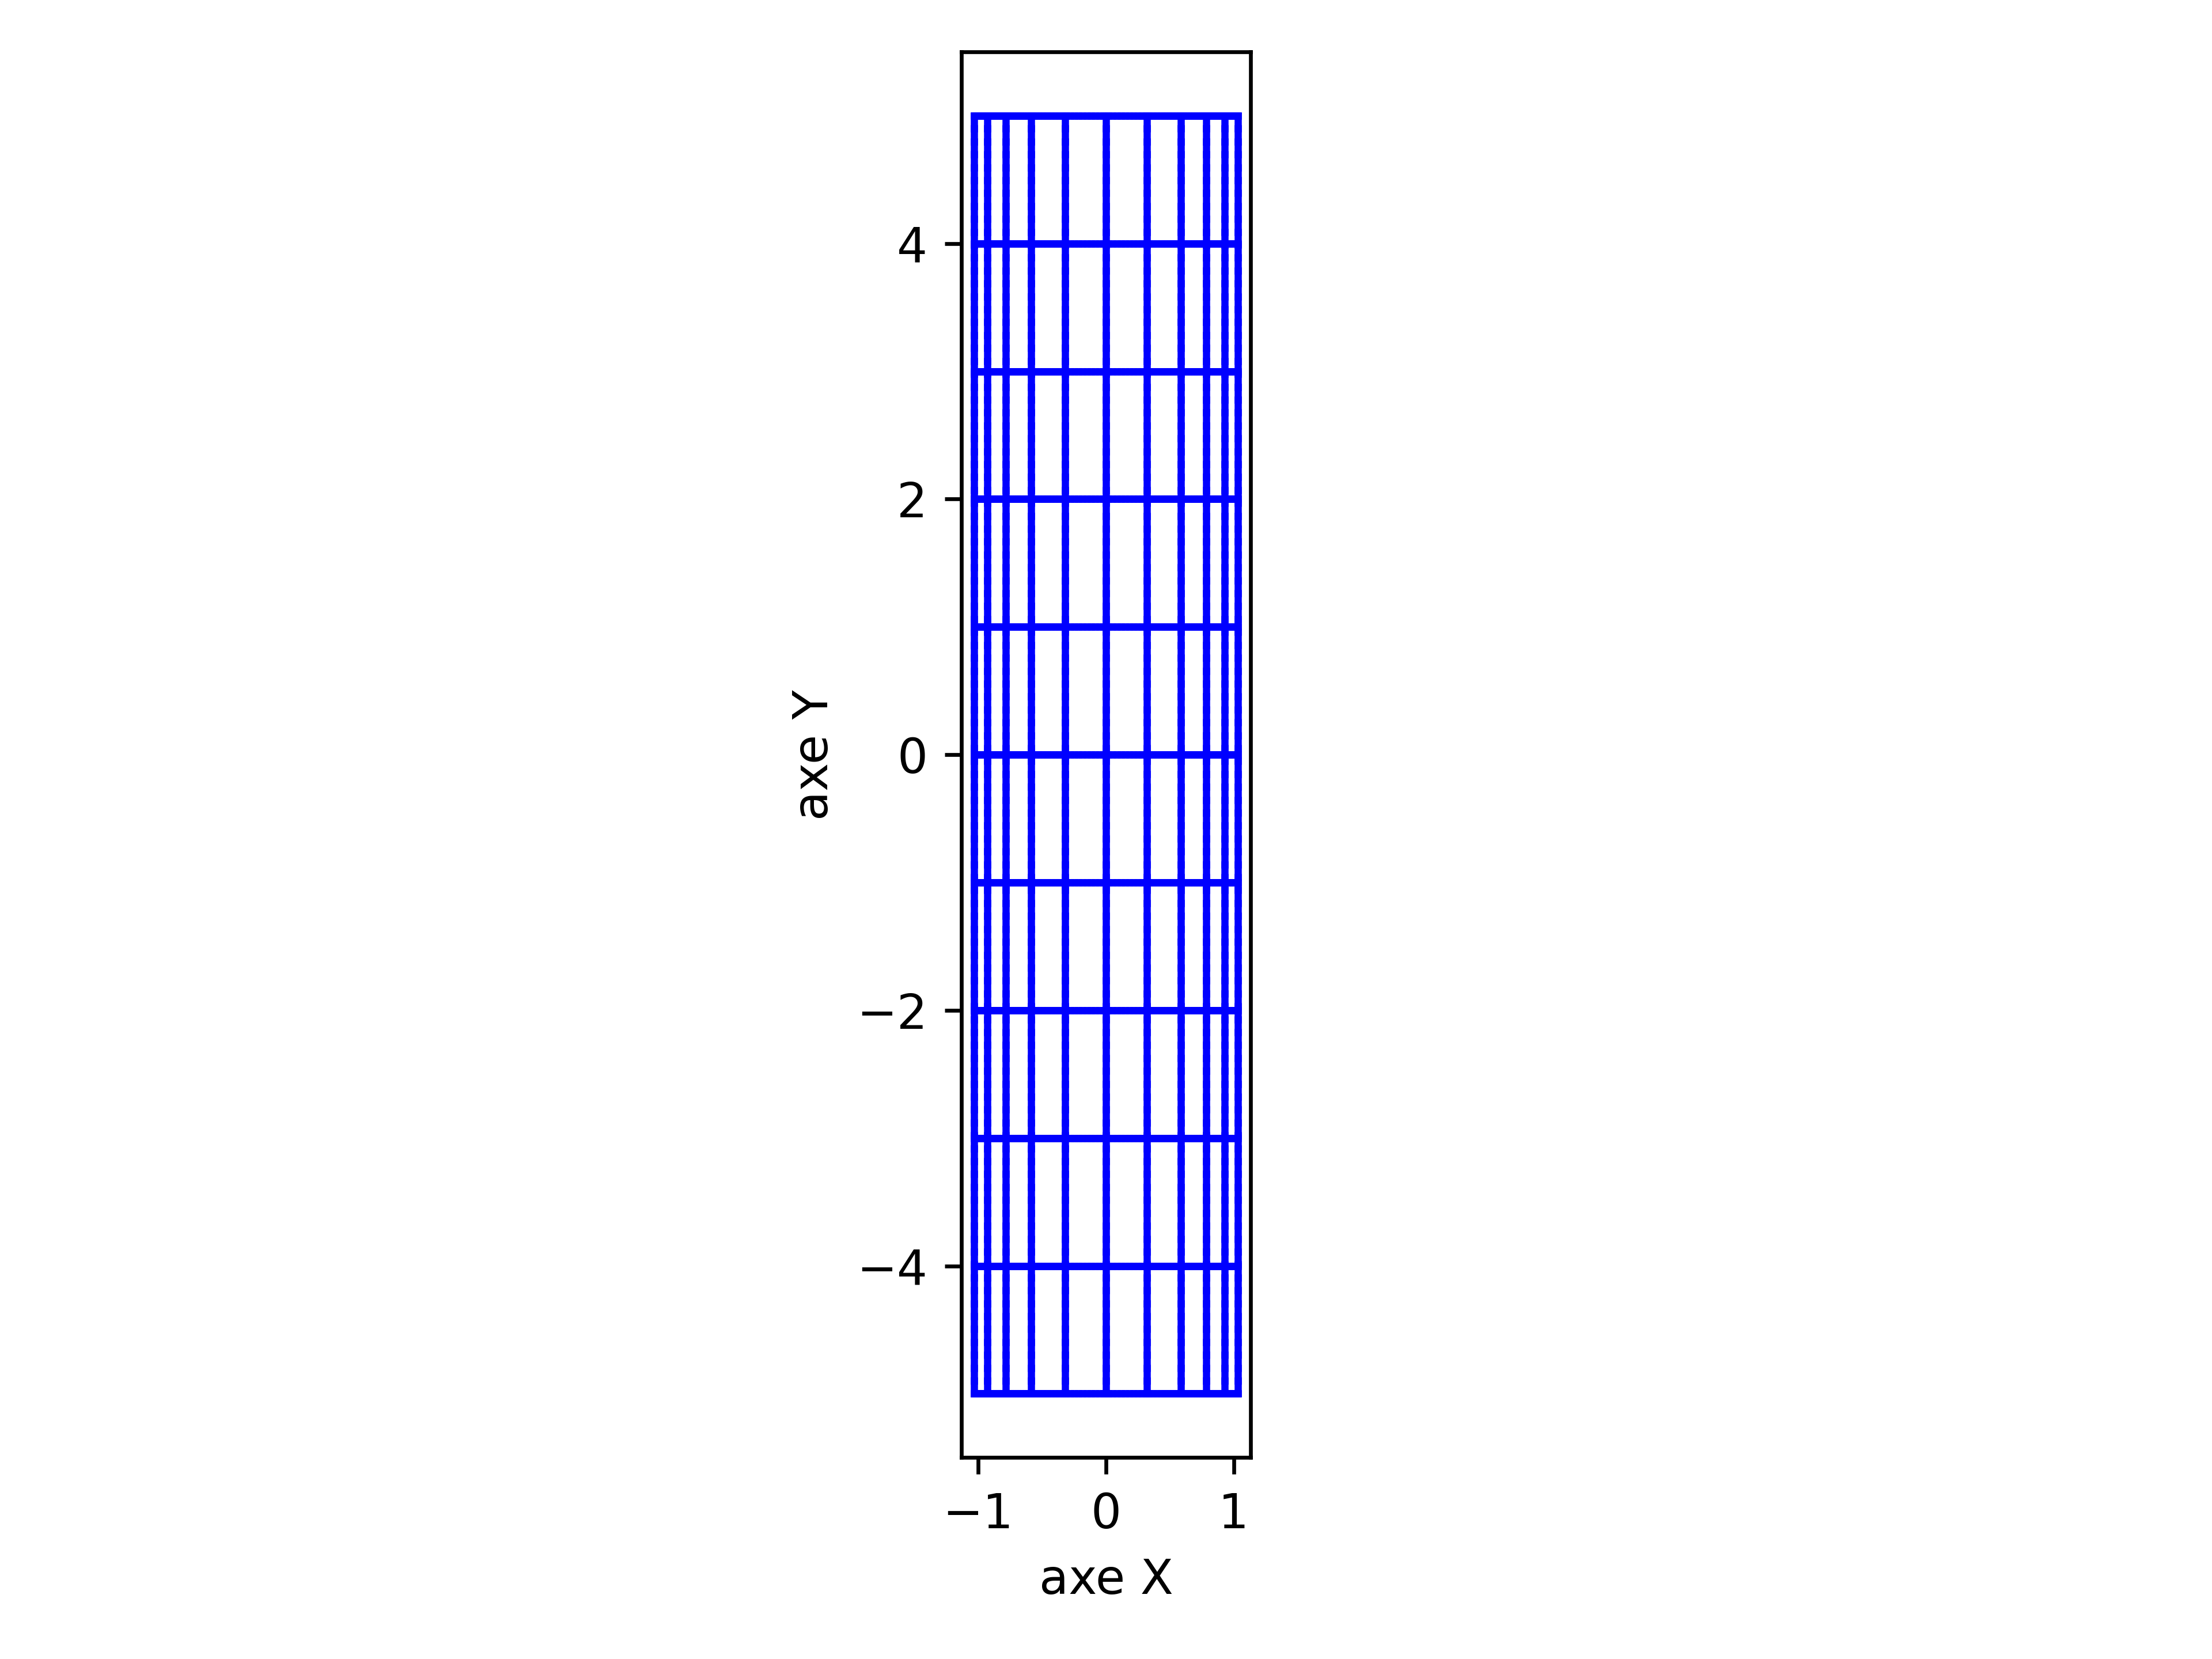
\includegraphics[scale=\myscale,scale=0.55,trim={3cm 0 3cm 0},clip]{figures/grille_coordonnees_cylindriques}	
	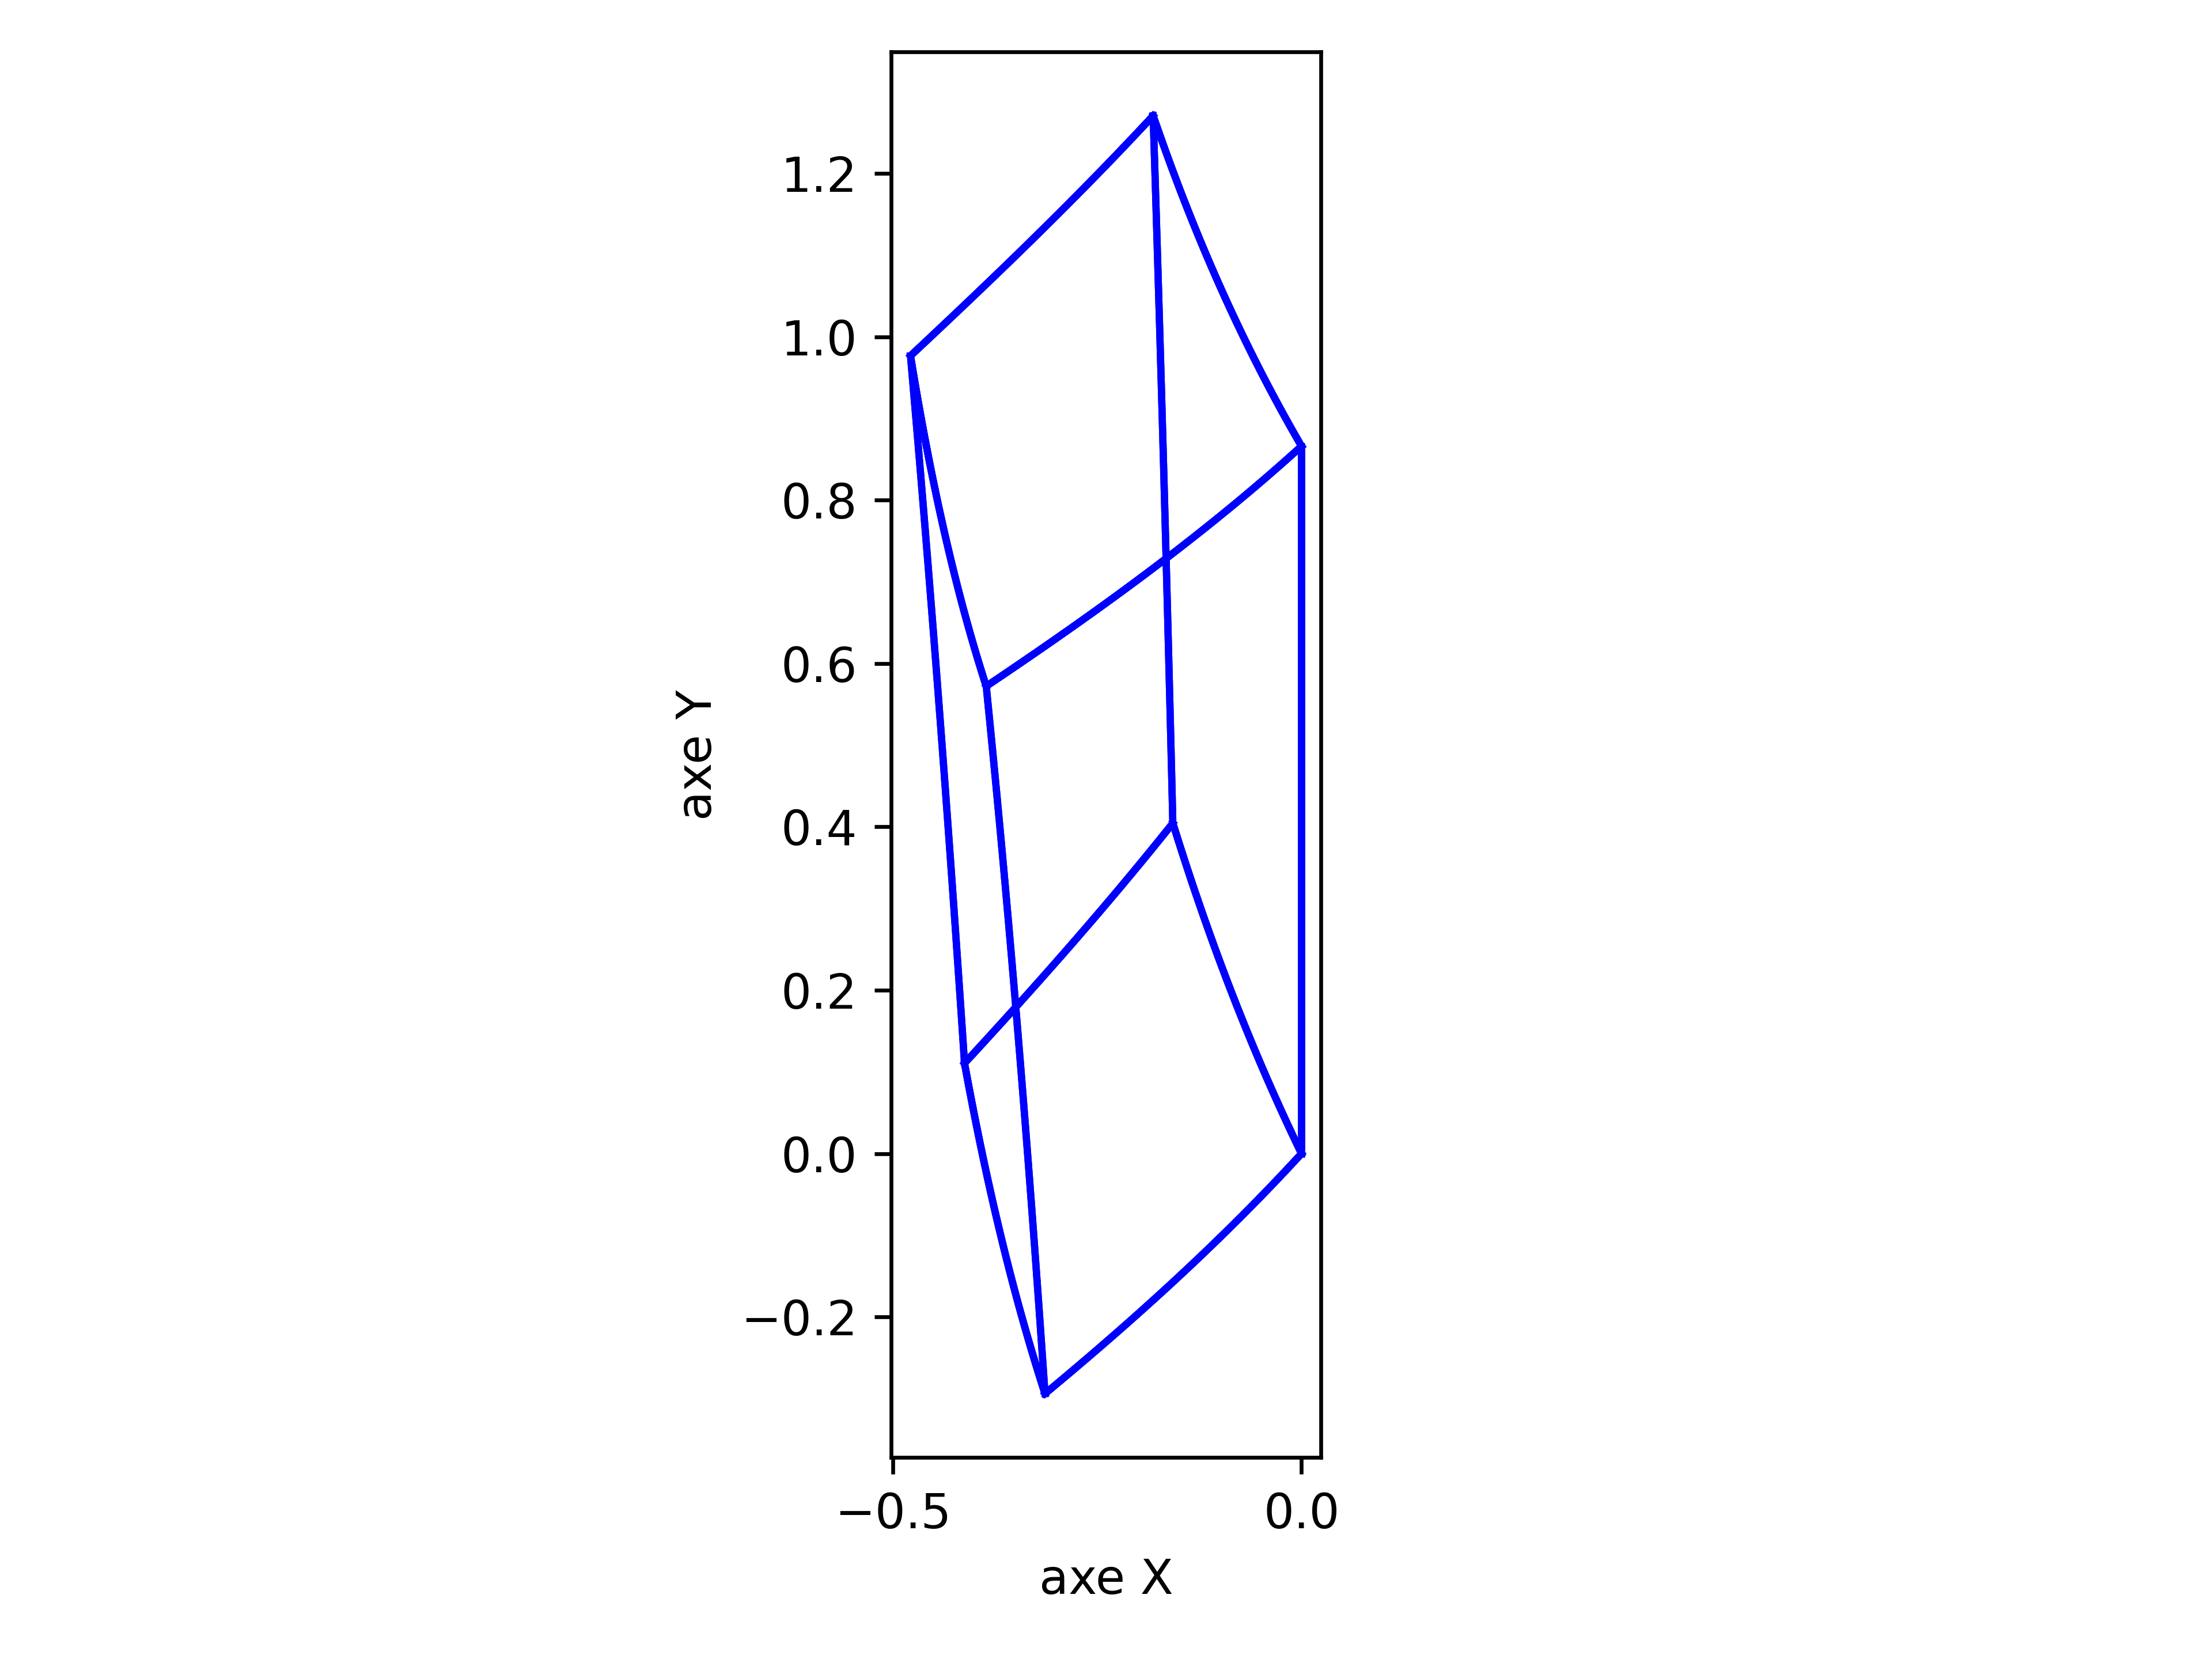
\includegraphics[scale=\myscale,scale=0.55,trim={3cm 0 3cm 0},clip]{figures/cube_coordonnees_cylindriques}
\end{center}

%--------------------------------------------------------------------
\subsection{Coordonnées sphériques}

\index{coordonnees@coordonnées!spheriques@sphériques}

\index{projection!spherique@sphérique}
	
\emph{Remarque.} On peut faire la même chose avec les coordonnées sphériques :
$$P(x,y,z) \longmapsto P(r,\varphi,\lambda) \longmapsto P'(X,Y) = (-\lambda,\varphi)$$
où $\varphi \in [-\frac\pi2,\frac\pi2]$  est la latitude et $\lambda \in ]-\pi,\pi]$ est la longitude.

\myfigure{0.3}{\tikzinput{fig-perspective-21}}

On pourrait imaginer beaucoup d'autres variantes, mais comme pour les projections cartographiques, aucune n'est parfaitement fidèle.

\begin{center}
	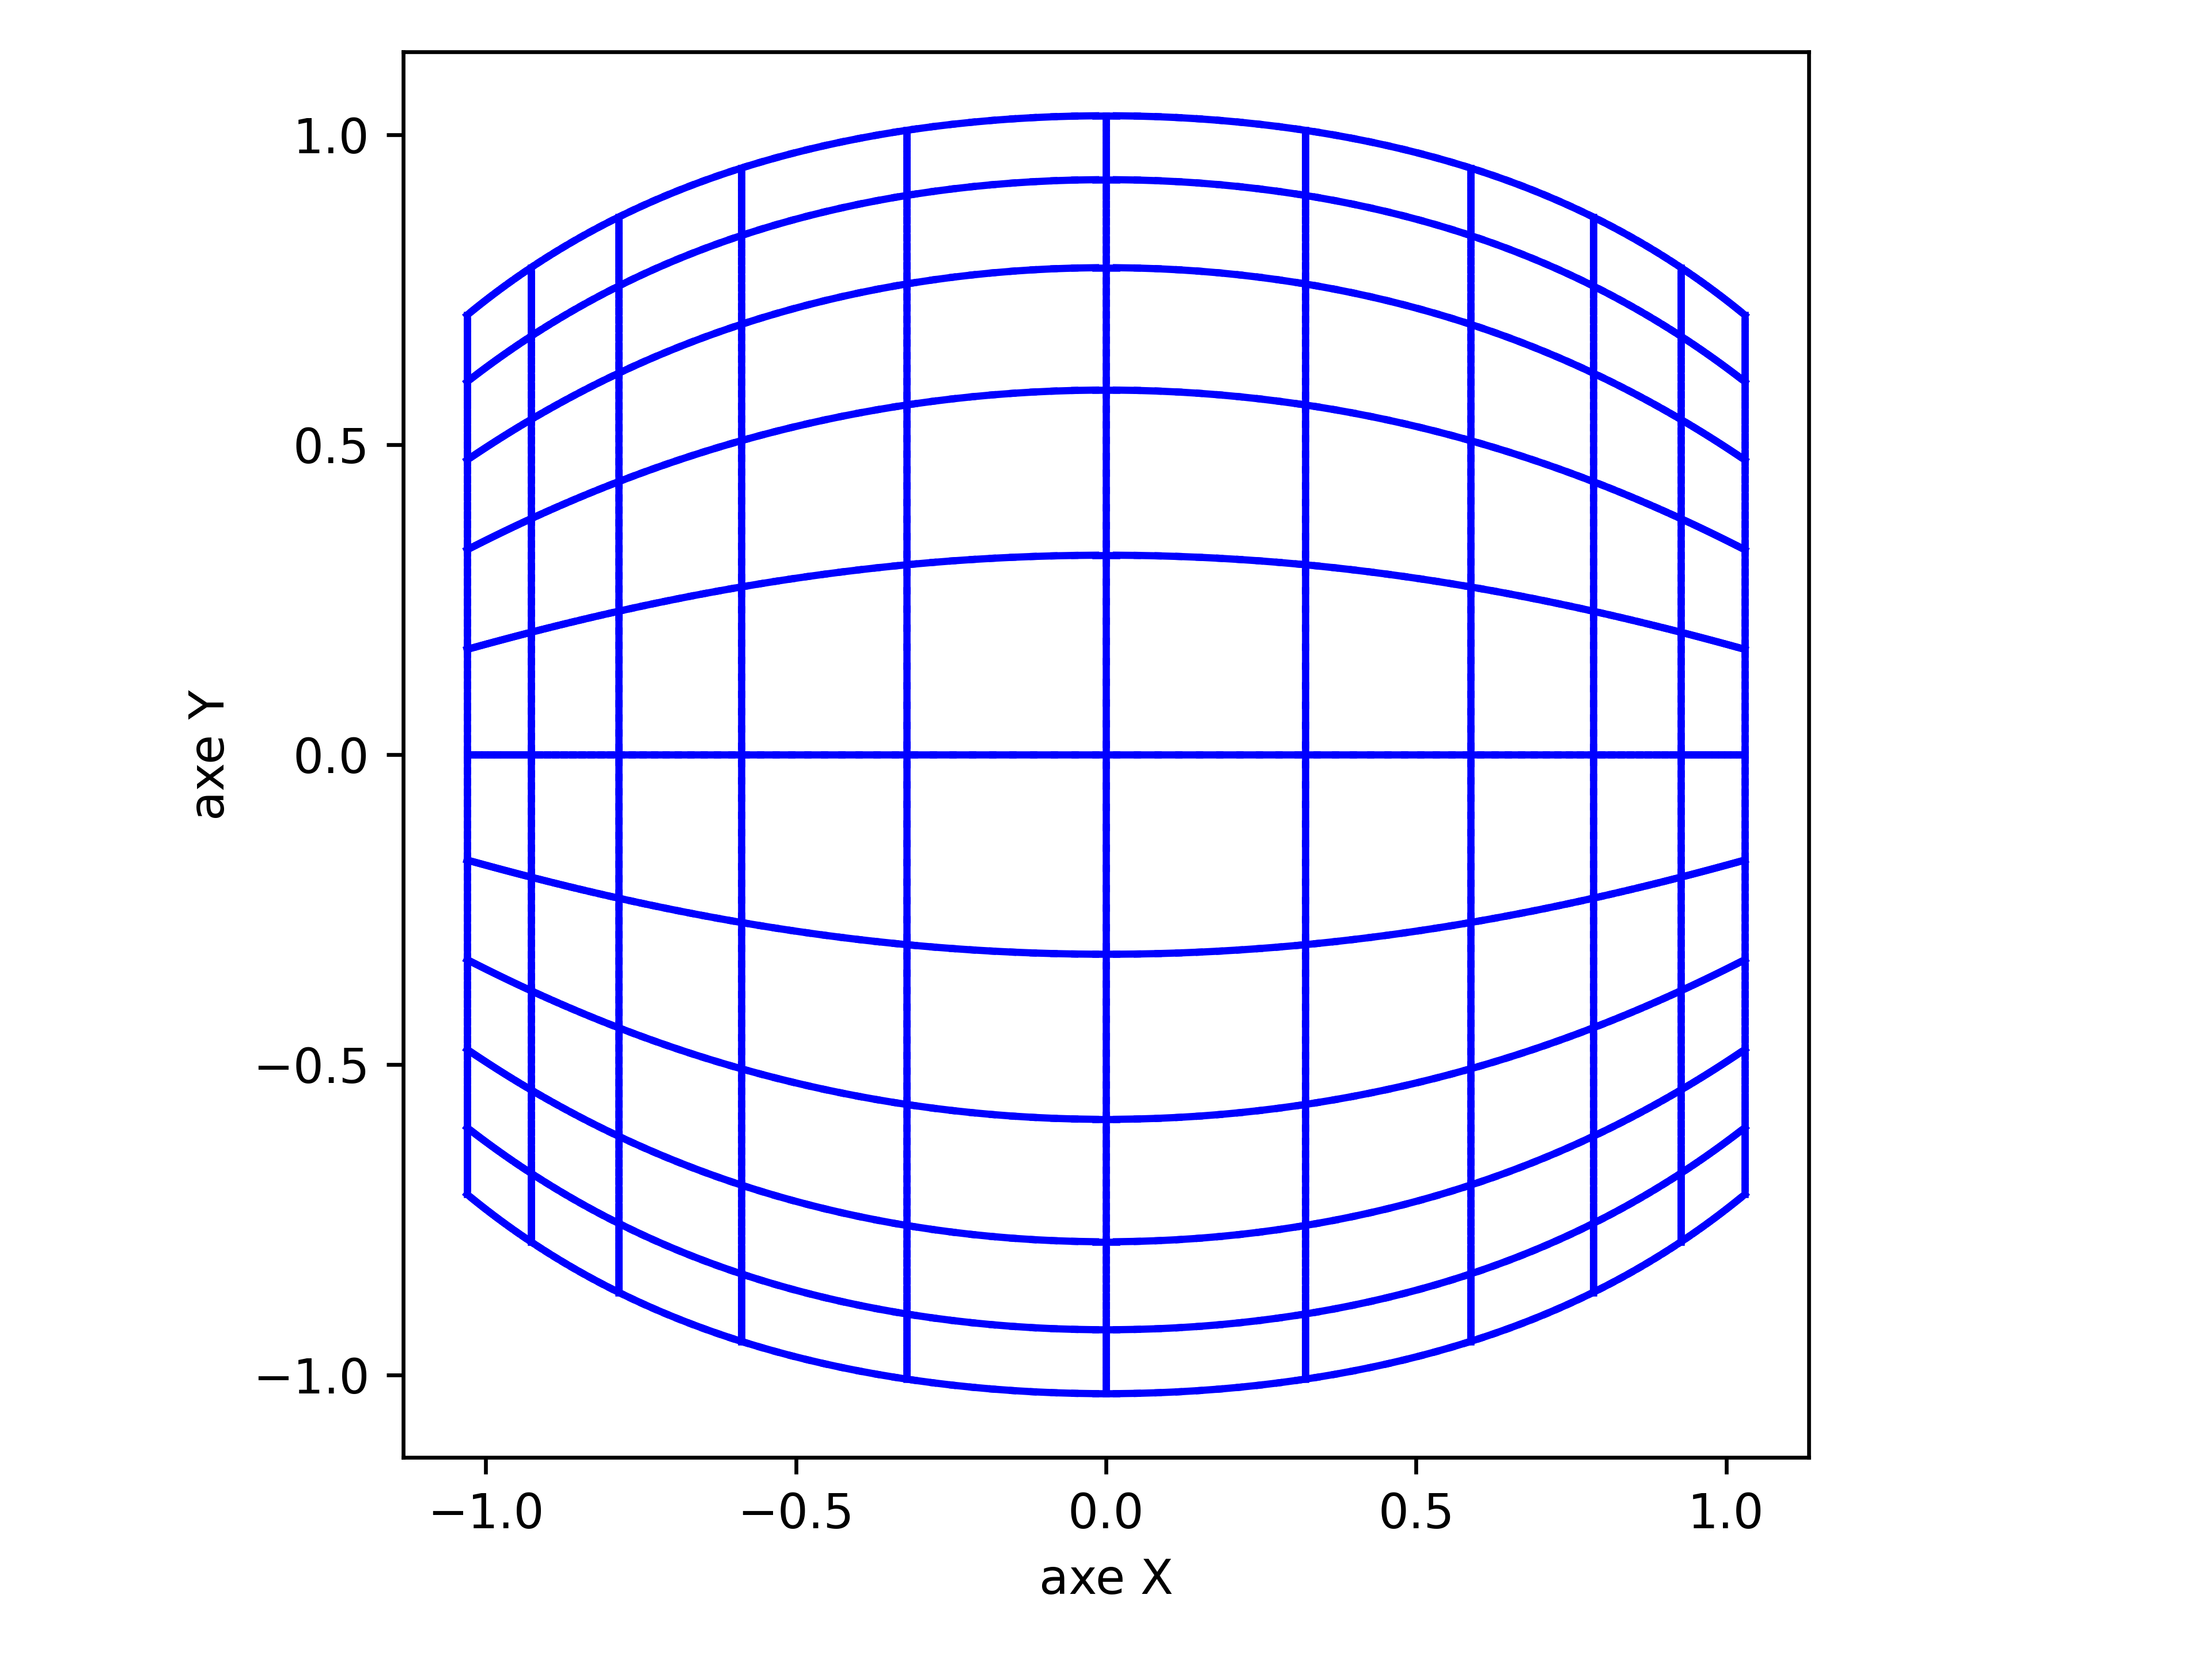
\includegraphics[scale=\myscale,scale=0.5]{figures/grille_coordonnees_spheriques}	
	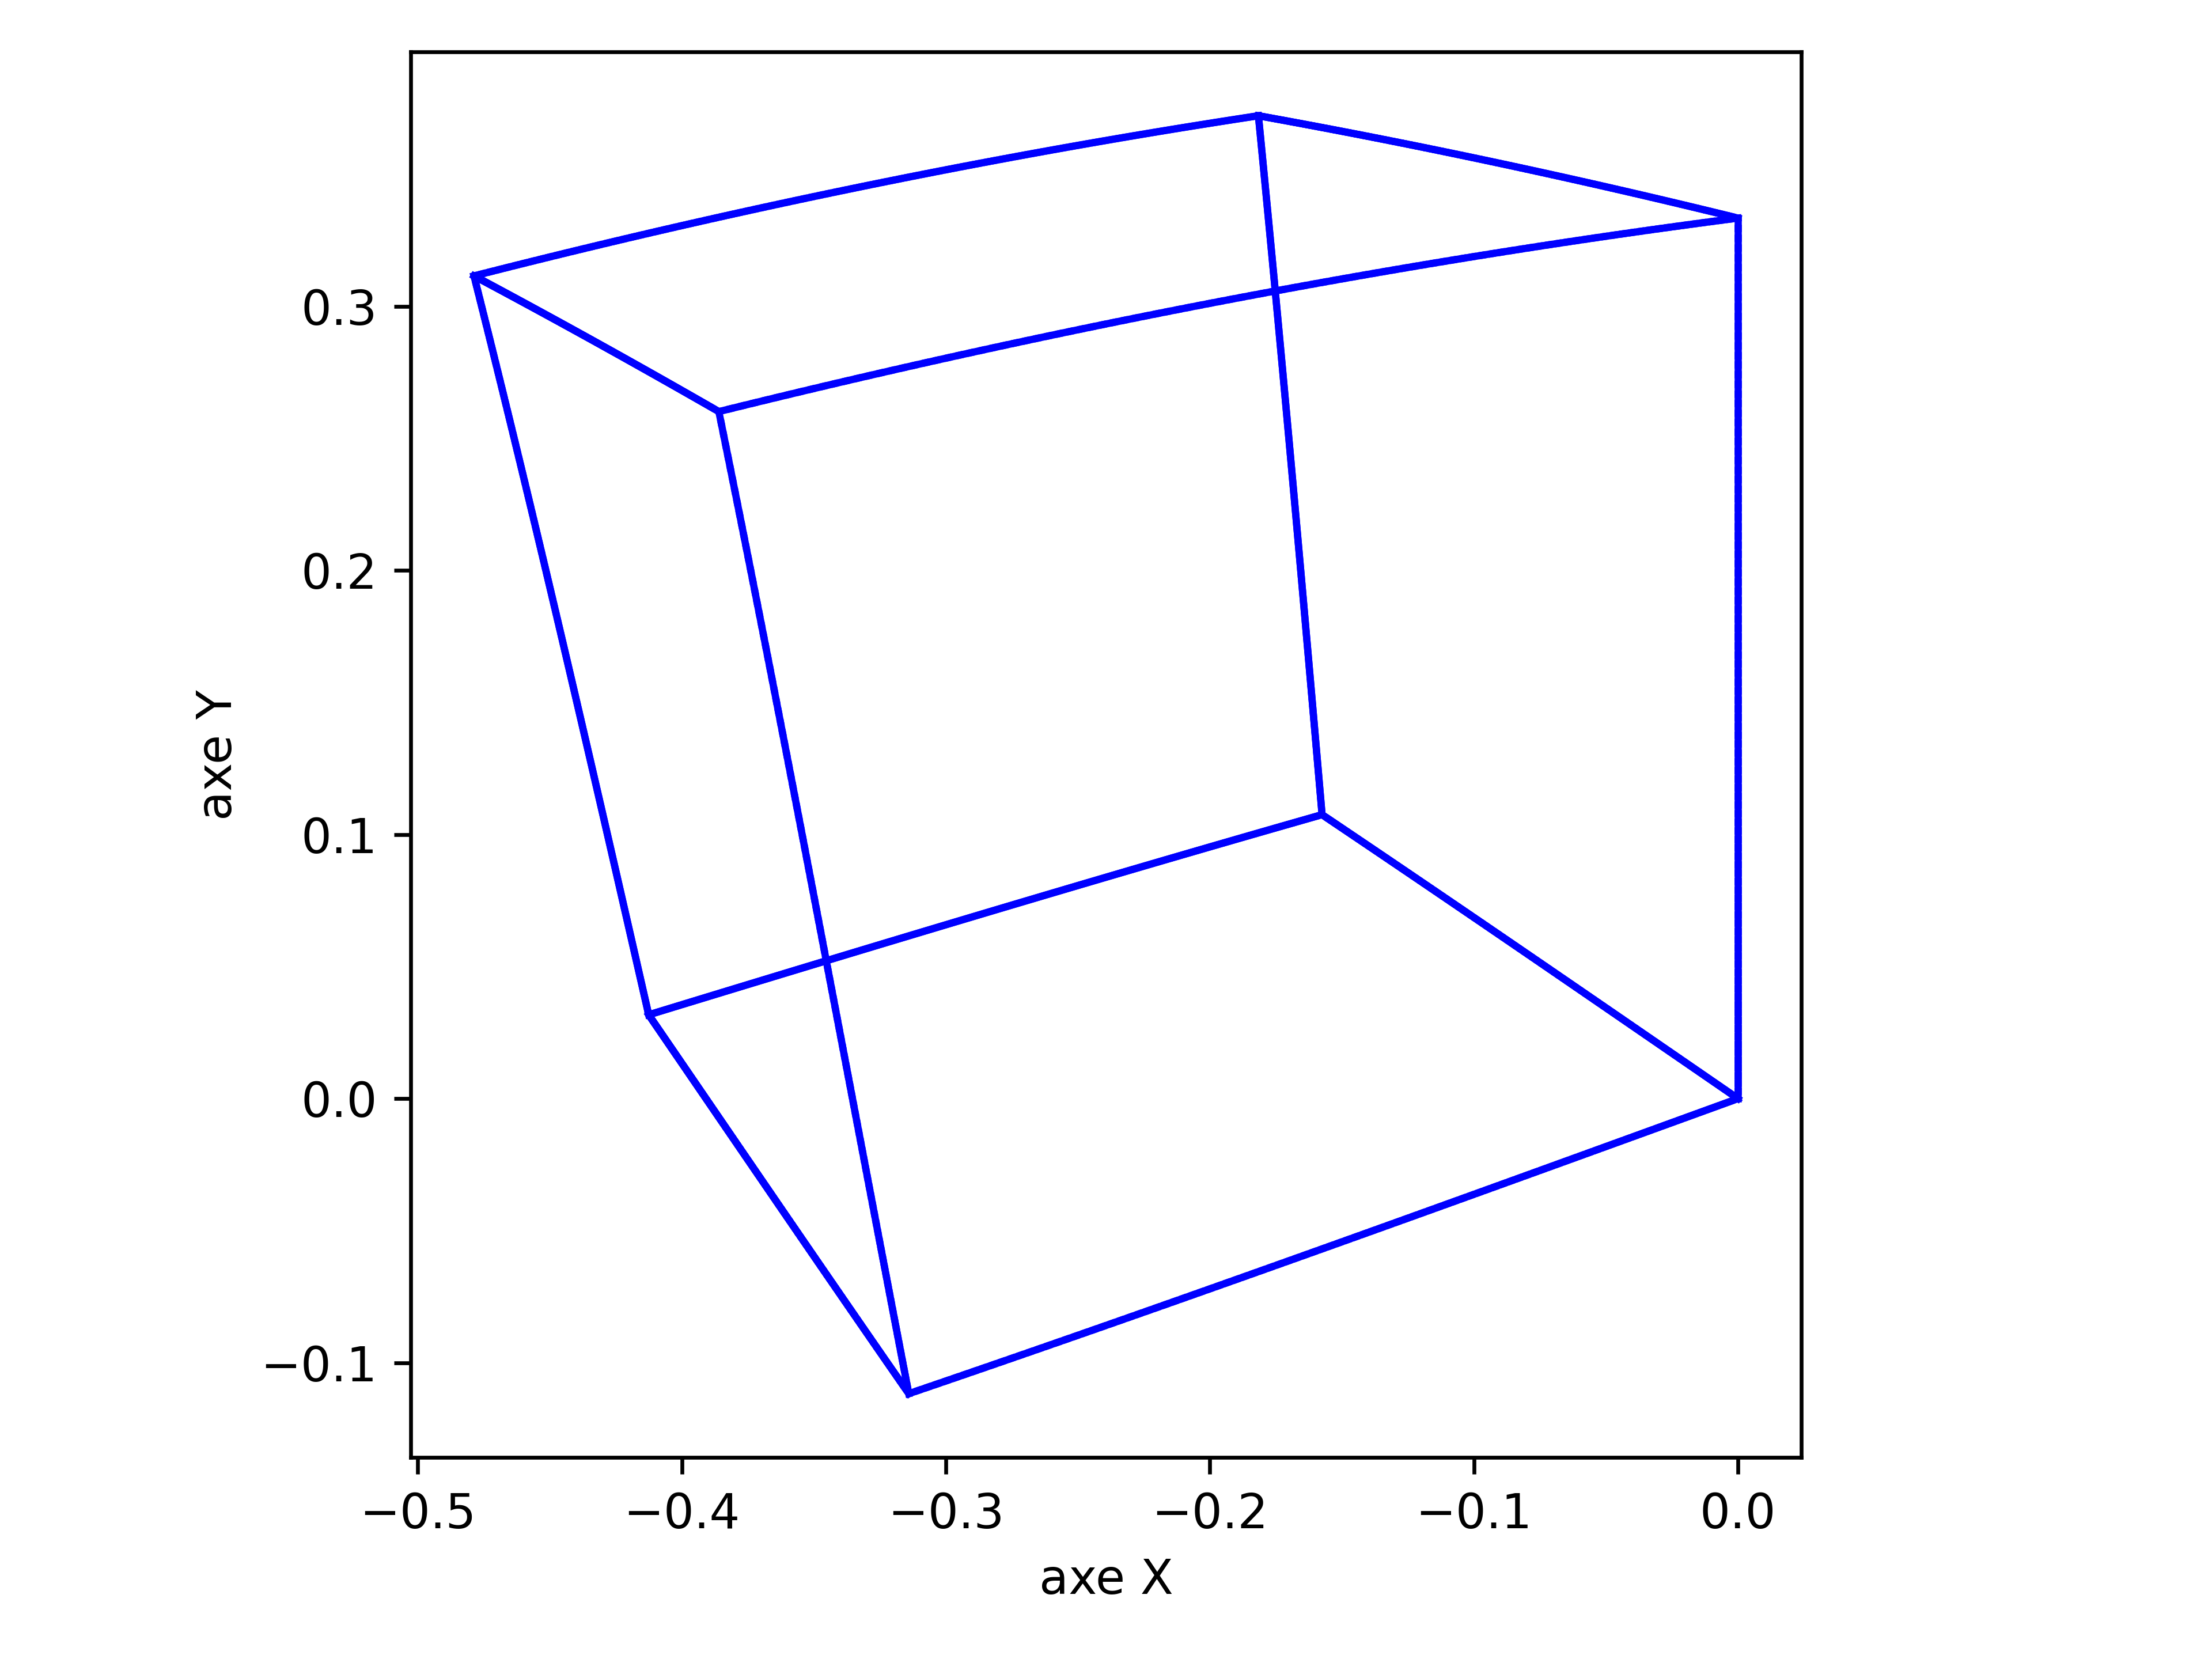
\includegraphics[scale=\myscale,scale=0.5]{figures/cube_coordonnees_spheriques}
\end{center}

%--------------------------------------------------------------------
\subsection{Perspective curviligne cylindrique}


La perspective curviligne cylindrique part du principe que dans une vision à \ang{180} les objets sur la droite et la gauche du champ de vision devraient paraître plus petits que les objets en face.

On considère un cylindre vertical, d'axe $(Oz)$, de rayon $R$. La projection s'effectue sur le plan vertical $\mathcal{P}$ d'équation $(x=R)$ tangent au cylindre.
La construction est la suivante : 
\begin{itemize}
  \item On part d'un point $P$ de l'espace,
  \item on le projette sur le point $P'$ du cylindre,
  \item puis on projette ce point orthogonalement sur le plan $\mathcal{P}$ en un point $P''$.
\end{itemize}

\myfigure{0.7}{\tikzinput{fig-perspective-22}}




Notons $P(x,y,z)$ les coordonnées du point à projeter et $r = \sqrt{x^2+y^2}$. La transformation est la suivante :
$$P(x,y,z) \longmapsto P'\left(x\frac{R}{r} , y\frac{R}{r} , z\right) \longmapsto P''(X,Y) = \left(y \frac{R}{r},z\right)$$

Cette transformation conserve la hauteur $z$ des points.

\begin{center}
	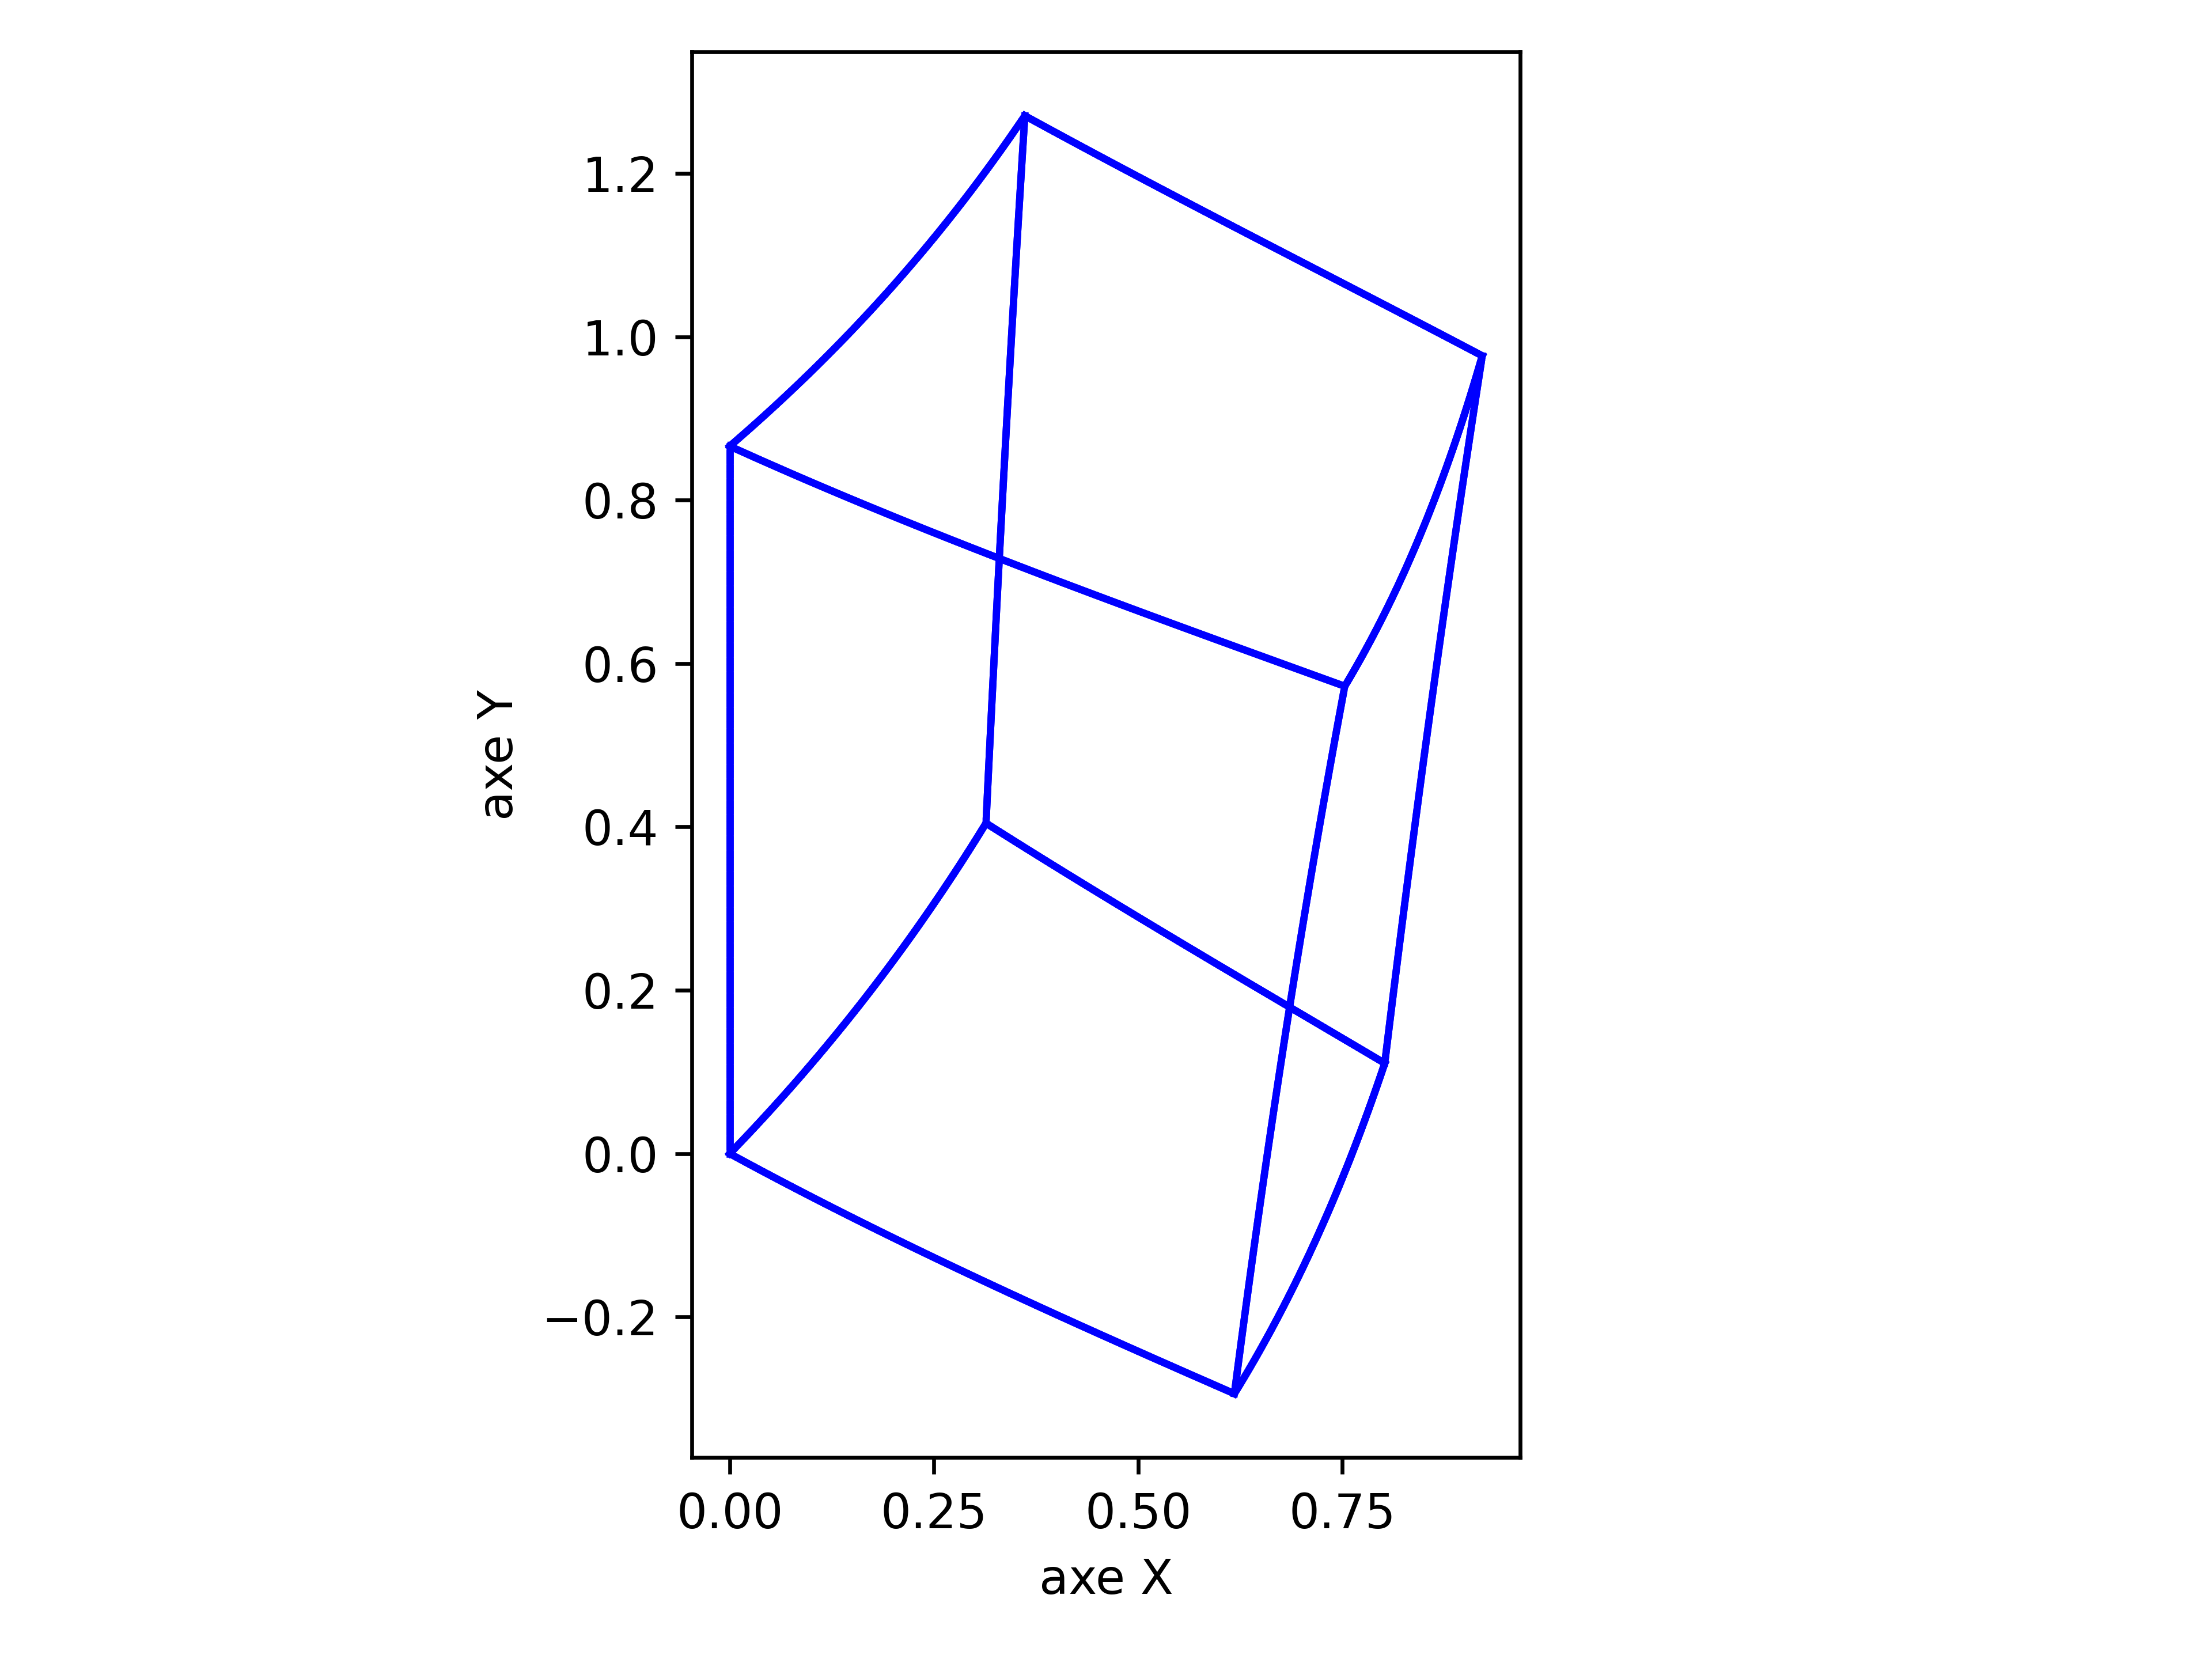
\includegraphics[scale=\myscale,scale=0.5]{figures/cube_curviligne_cylindrique}
	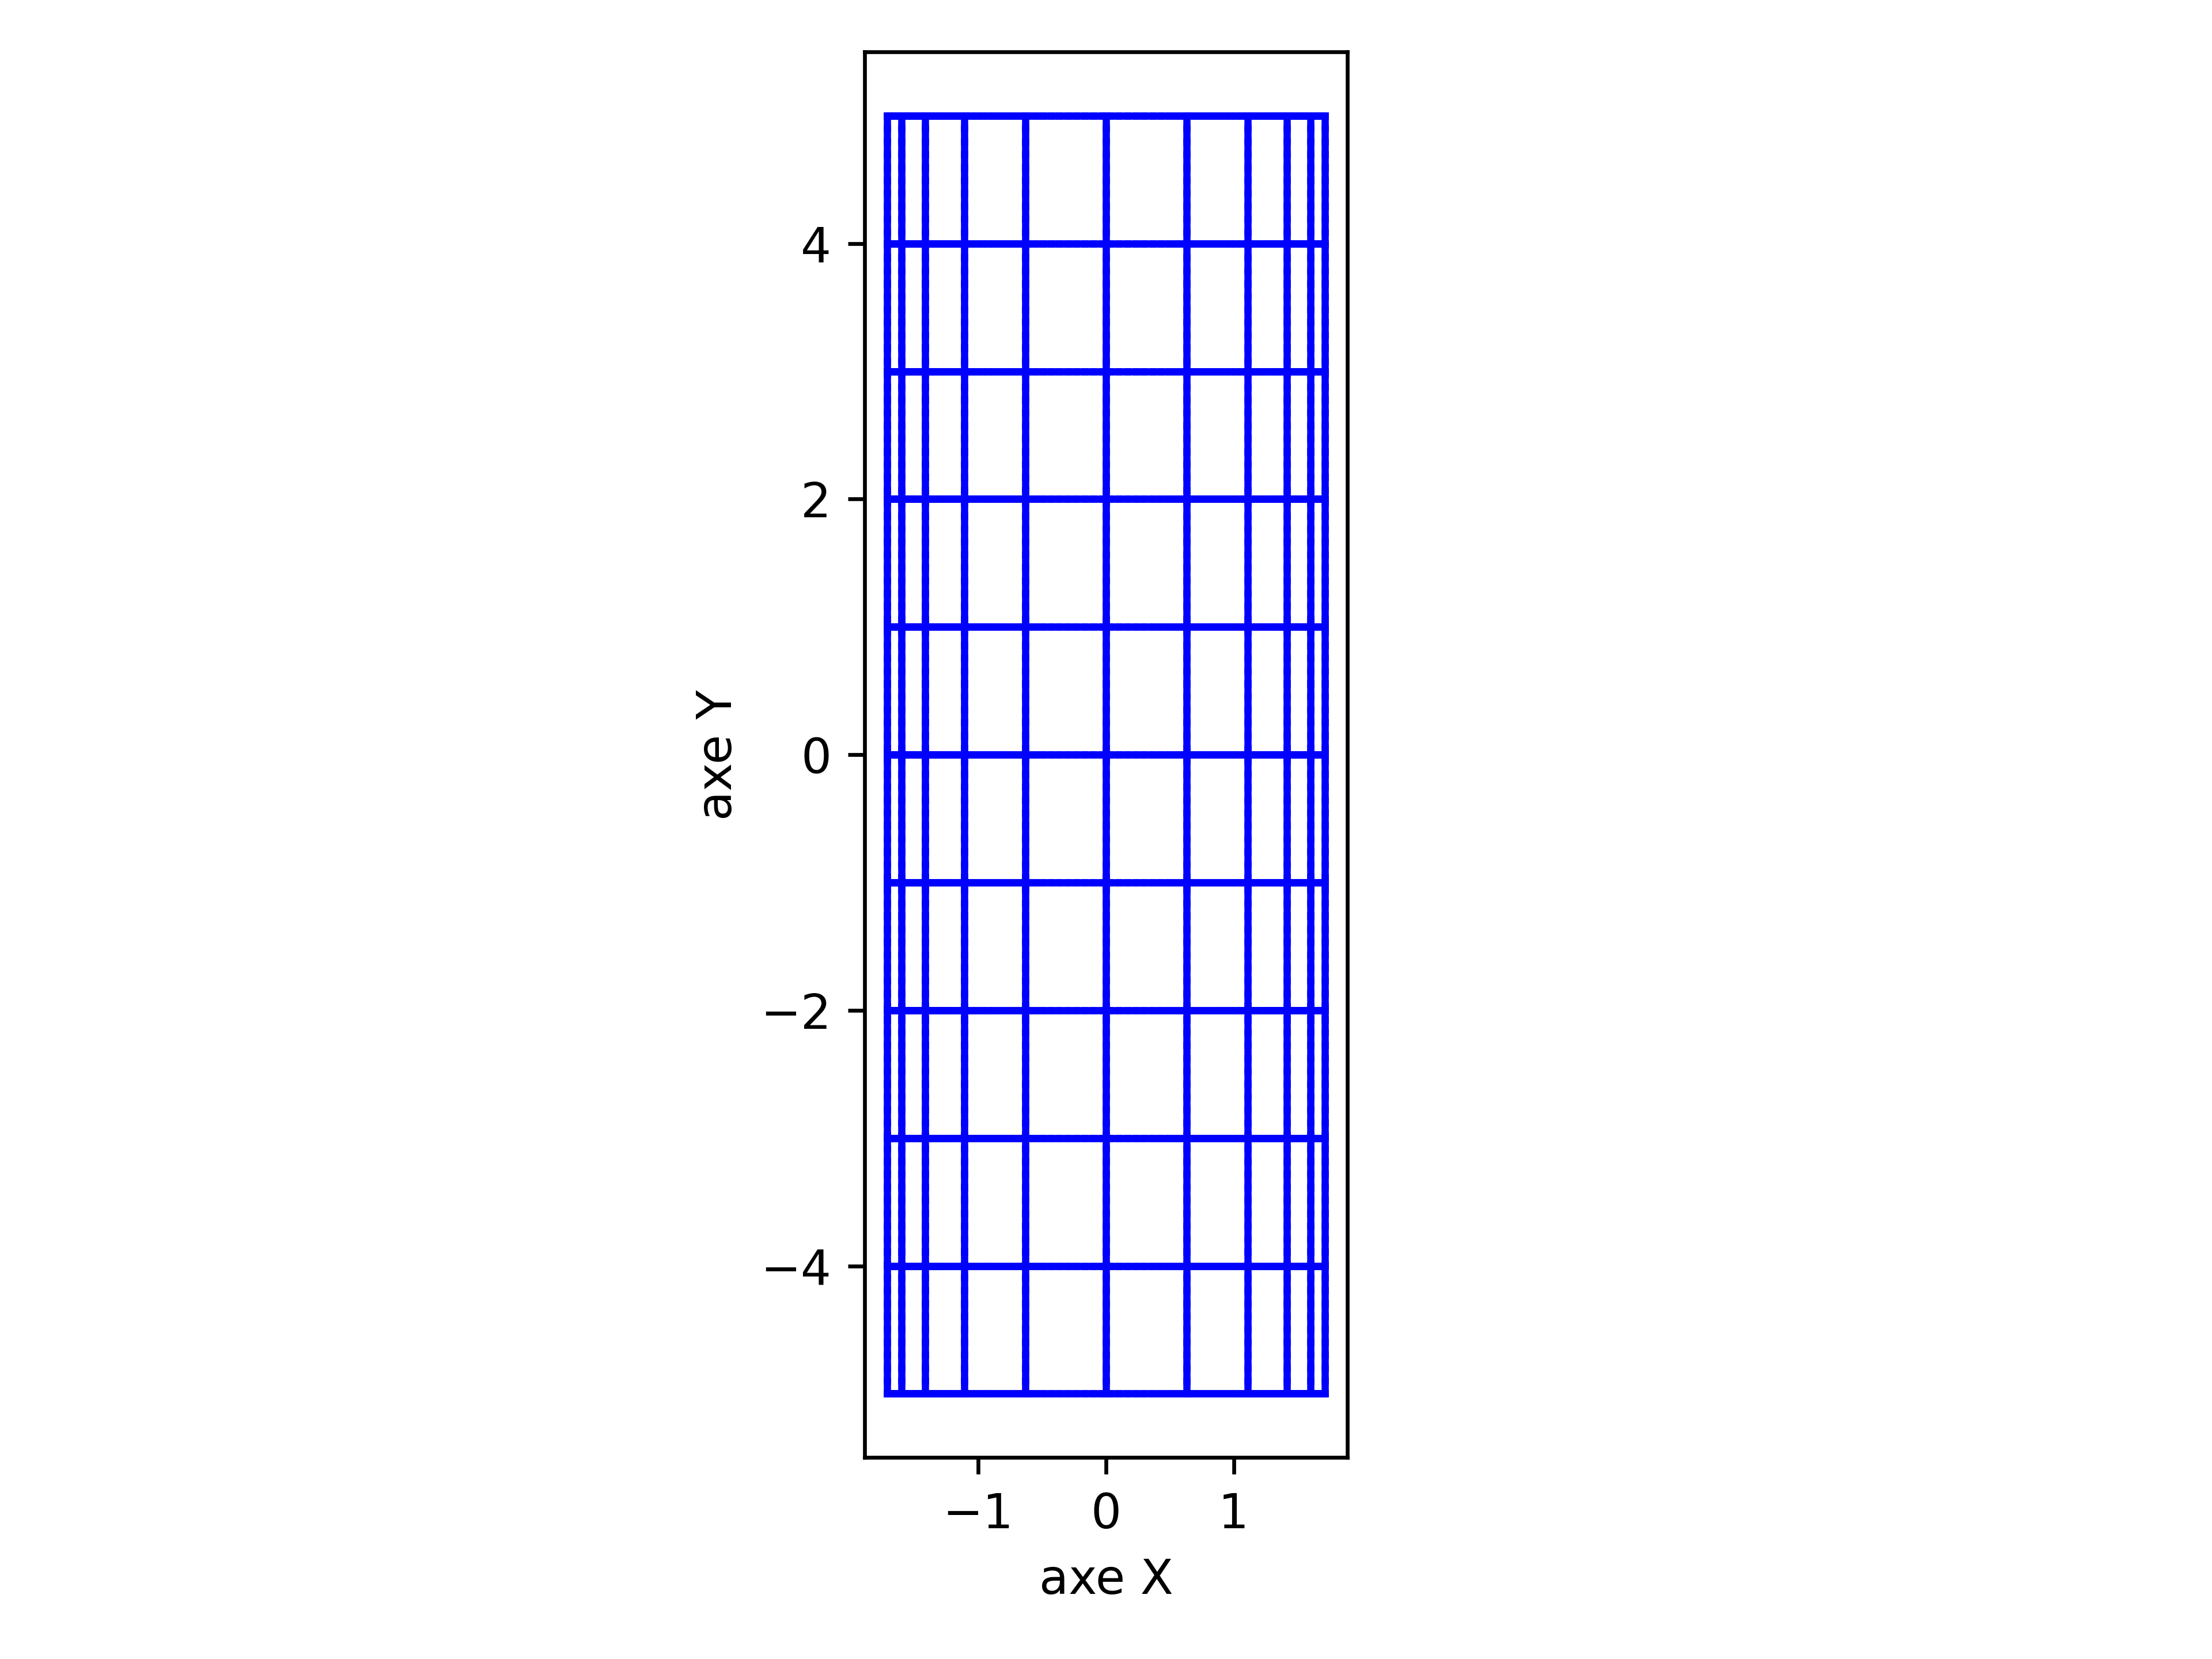
\includegraphics[scale=\myscale,scale=0.5]{figures/grille_curviligne_cylindrique}
\end{center}


%--------------------------------------------------------------------
\subsection{Perspective curviligne sphérique}

On étend la construction précédente sur le même principe avec une distorsion haut/bas, en plus de la distorsion gauche/droite. On obtient une vue à \ang{180} de gauche à droite, mais aussi de haut en bas.
Le résultat obtenu ressemble à une photographie prise avec un objectif de type \emph{fisheye}.

Dans cette construction, on projette le point sur une (demi-)sphère de rayon $R$, puis sur un plan vertical tangent.




Pour $P(x,y,z)$ on note cette fois $r = \sqrt{x^2+y^2+z^2}$.
La transformation est :
$$P(x,y,z) \longmapsto P'\left(x \frac{R}{r},y \frac{R}{r}, z\frac{R}{r}\right) \longmapsto P''(X,Y) = \left(y \frac{R}{r},z \frac{R}{r}\right)$$


\begin{center}
	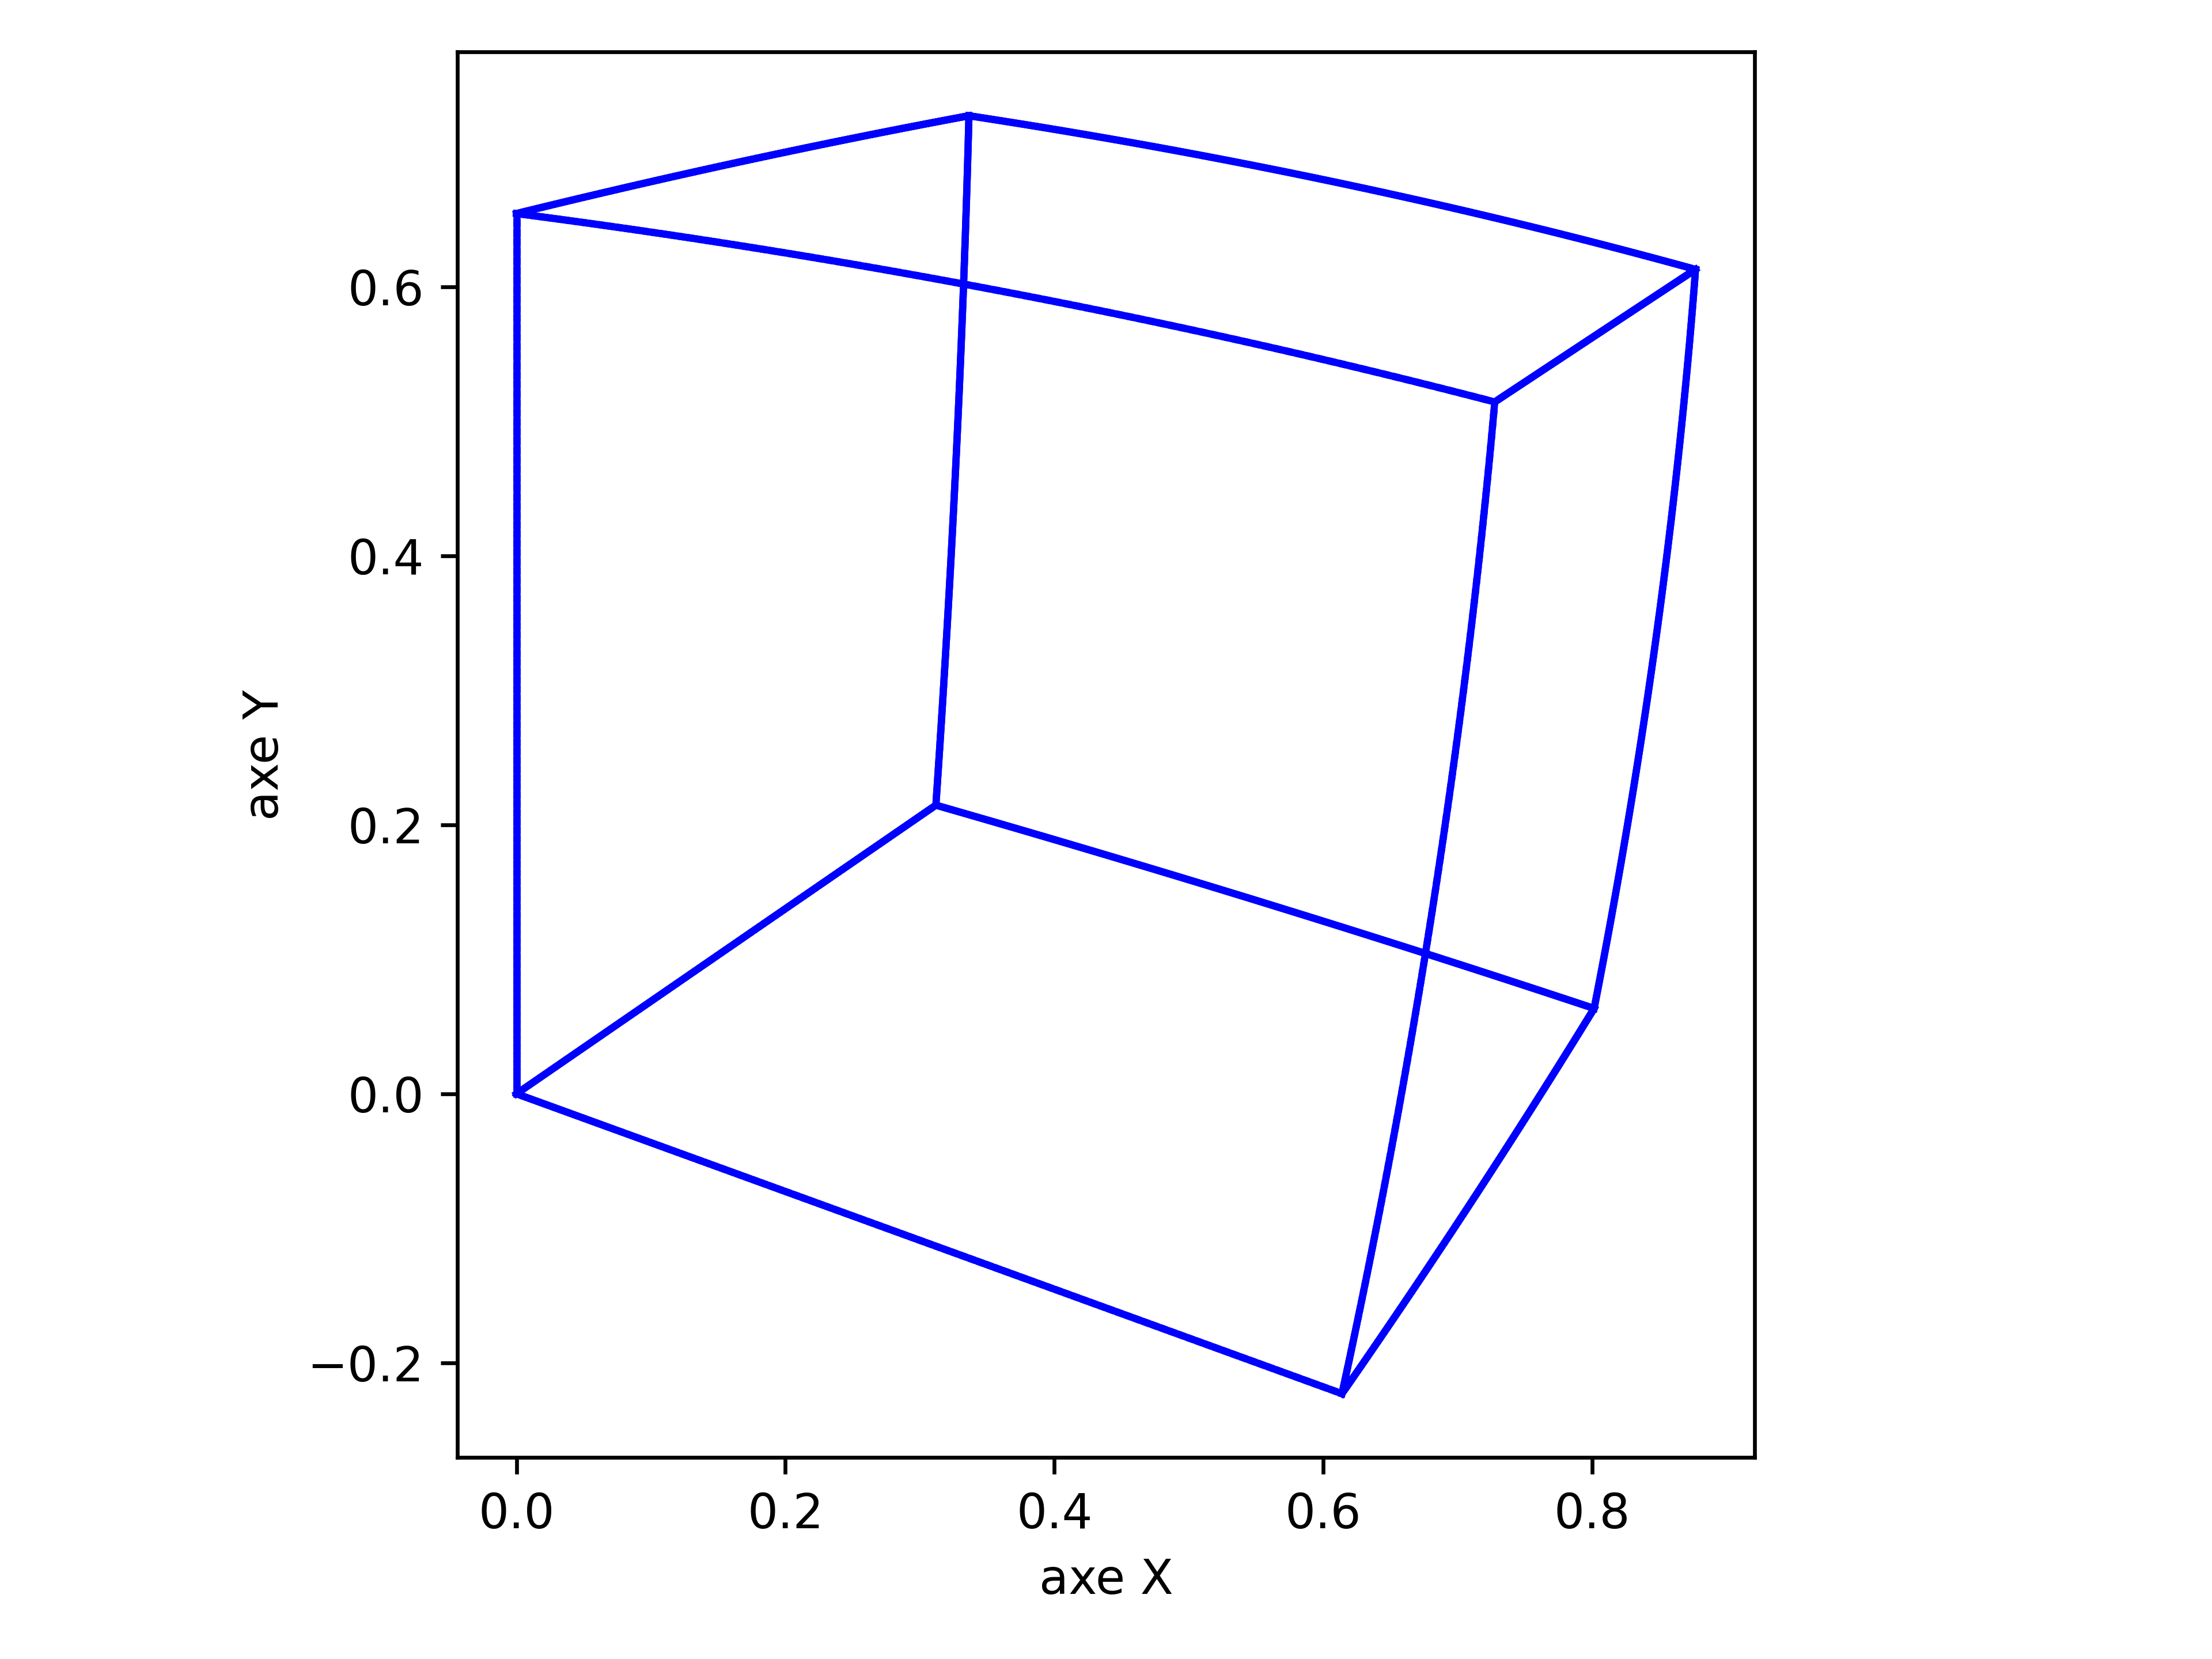
\includegraphics[scale=\myscale,scale=0.5]{figures/cube_curviligne_spherique}
	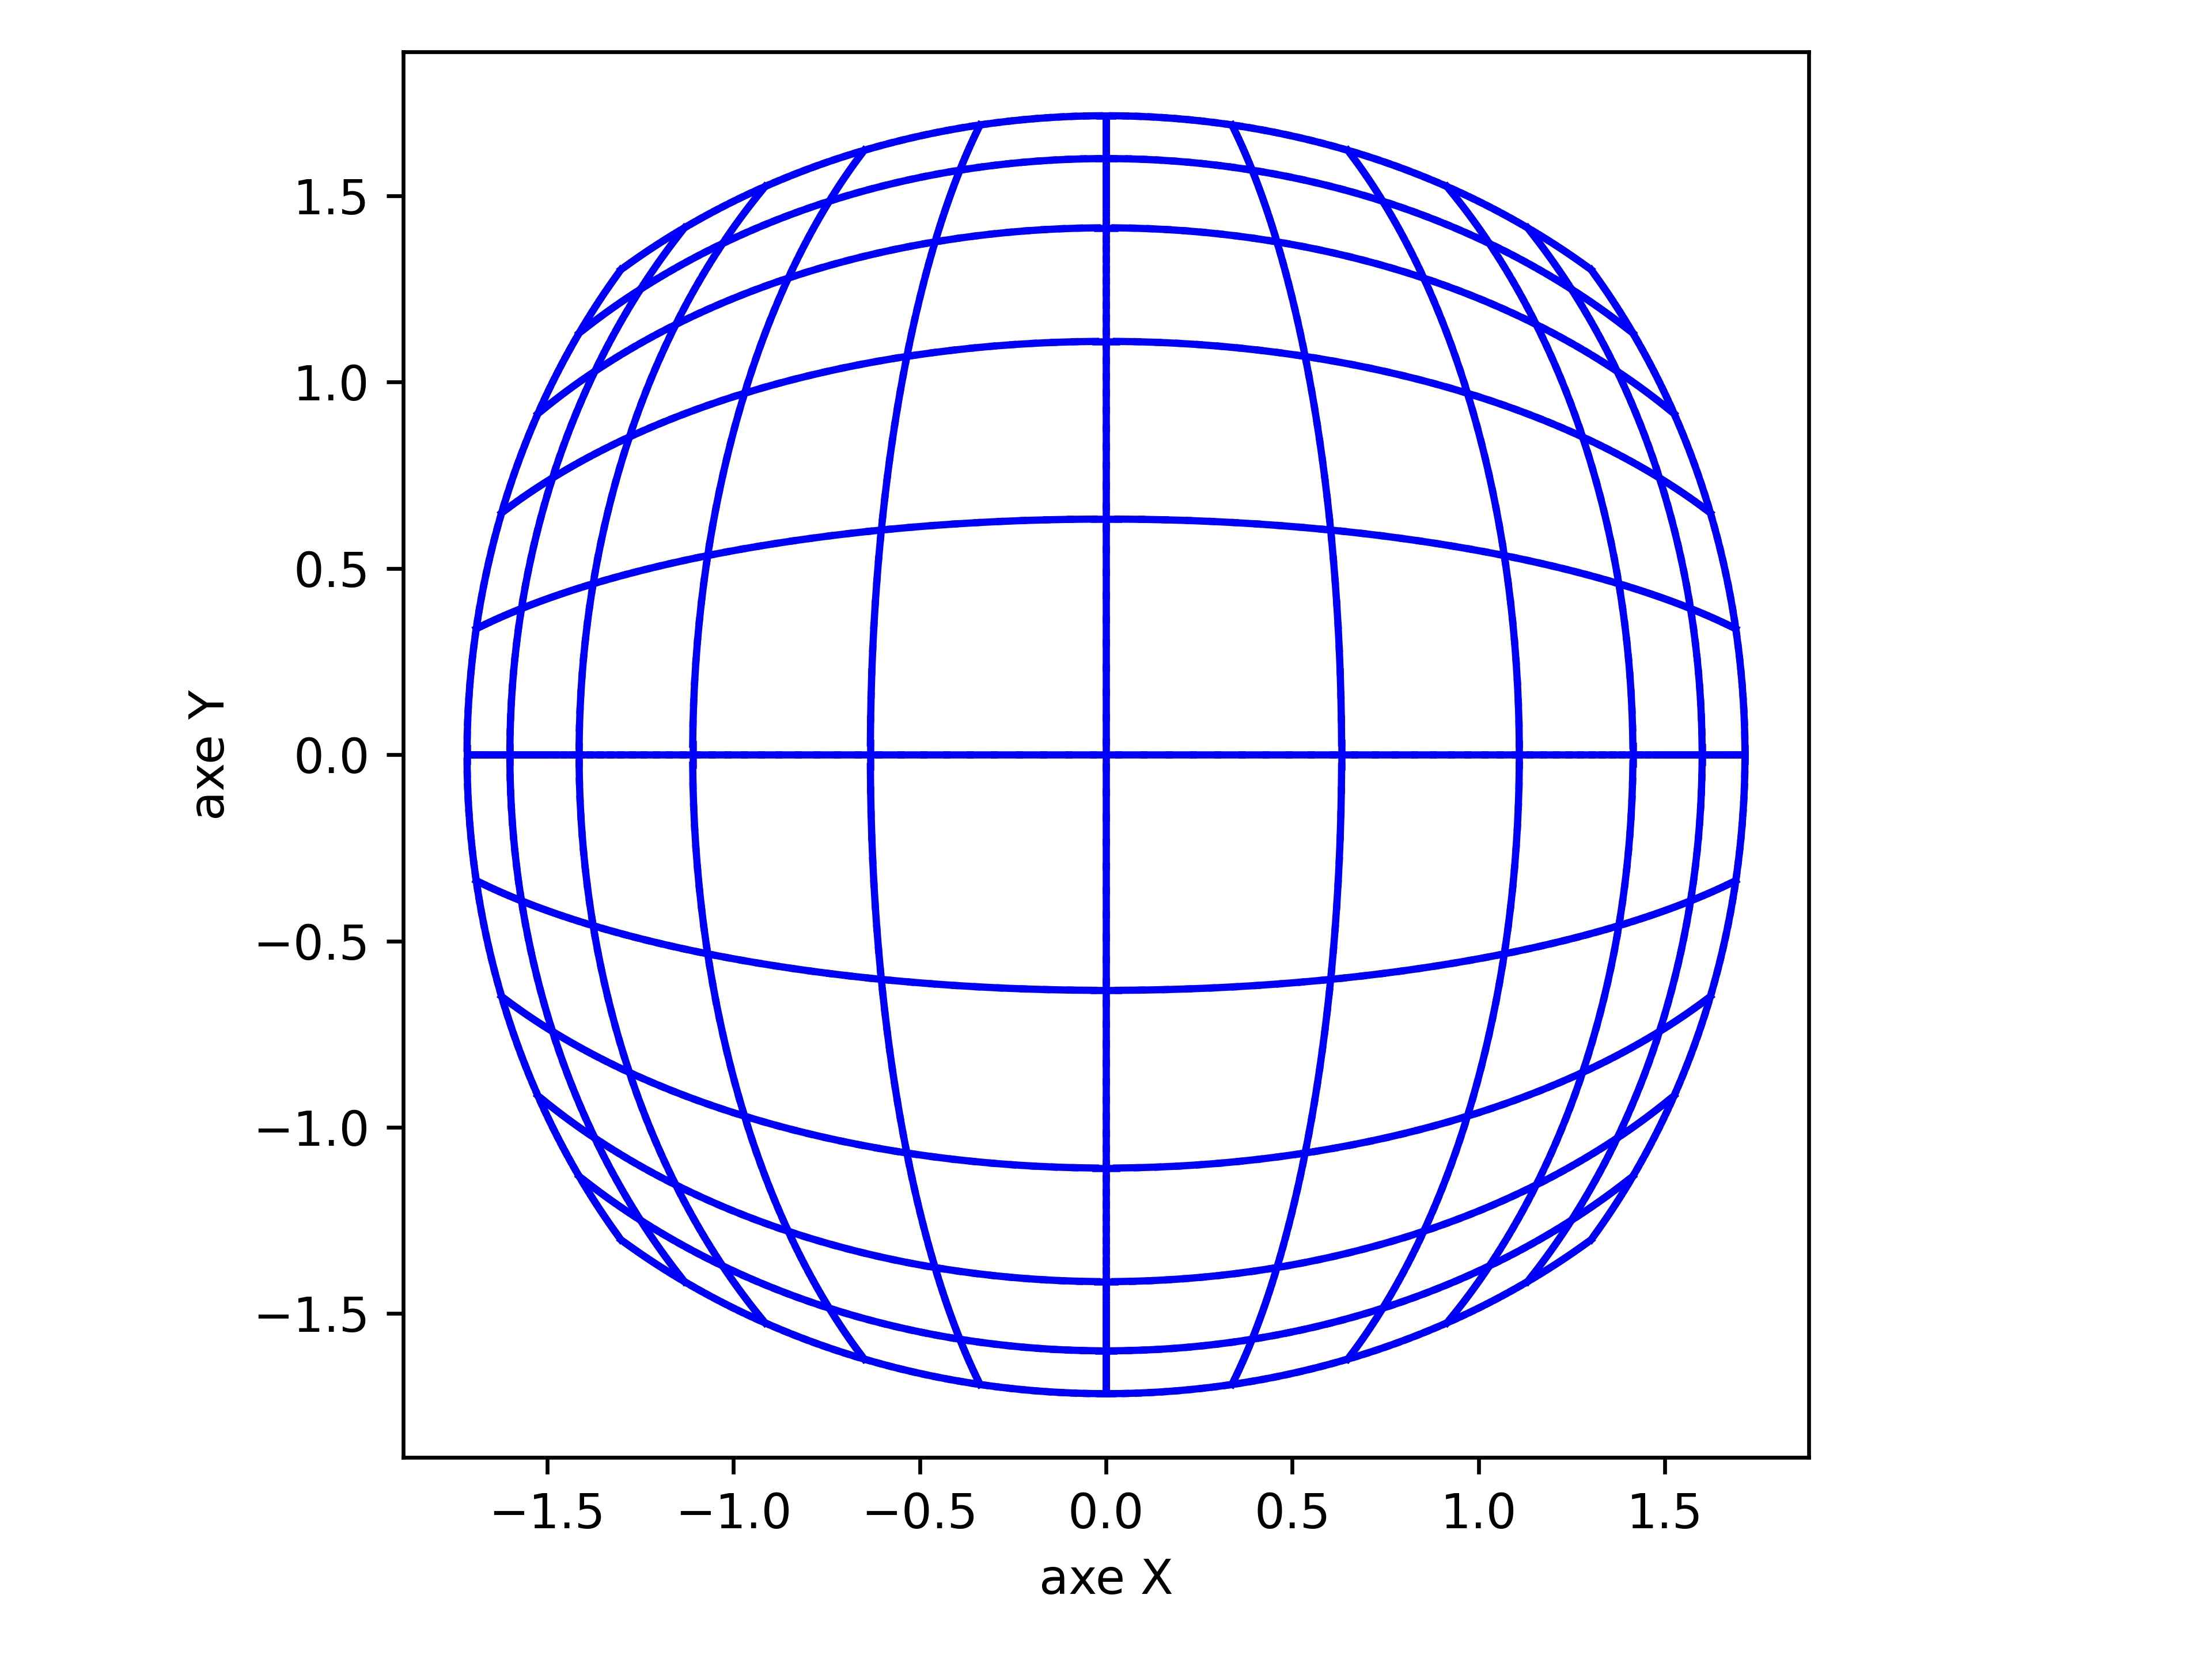
\includegraphics[scale=\myscale,scale=0.5]{figures/grille_curviligne_spherique}
\end{center}

\bigskip
\bigskip
\bigskip


\end{document}
